\newcommand{\Li}{$^{8}$Li }
\renewcommand{\bf}{\bfseries}

\chapter{Cherenkov Optical Calibration Source for SNO+}
\label{ch:chsrc}

\label{chap:execsummary}

SNO+ has over 9500 Photo-Multiplier Tubes (PMTs) which detect light produced inside the target (water or liquid scintillator). Within the SNO+ calibration plan~\cite{gann:2013}, it is vital to extract and monitor the overall light collection efficiency. This can be achieved by deploying a source that produces a well understood and easily simulated optical signal. The SNO+ Cherenkov source is designed to produce this signal through tagged Cherenkov events. It is based on the SNO \Li source design and experience~\cite{Tagg:2002,Tagg:2001}.

%\begin{figure}
%\center{\includegraphics[width=.8\textwidth]
%{AnnotatedSource.png}}
%\caption{\label{fig:source_design2} The Cherenkov source design.}
%\end{figure}

As was done for the SNO \Li source, the \Li (t$_{1/2}$=0.838\,s) isotope is created using the available deuterium-tritium neutron generator in conjunction with a $^{11}$B target. The \Li is transported by helium gas to the Cherenkov source decay chamber, see Figure~\ref{fig:design-1}. The energetic beta particles produced by the decay are stopped in the 6\,cm-thick acrylic wall and produce Cherenkov light. The alphas from the subsequent $^{8}$Be decay produce scintillation light in the helium. A small PMT in the neck of the source detects this scintillation light, generating a tagging signal for the event. 

The Cherenkov source decay chamber is made from UV-absorbent (UVA) acrylic in order to block the UV component of the Cherenkov light. Thus, the remaining light that propagates through the SNO+ detector is quasi-independent of the optical properties of the LAB-PPO scintillator. The alpha scintillation light must be contained within the decay chamber to prevent contamination of the Cherenkov light. A black (carbon) opaque lining is therefore deposited on the inside of the decay chamber. On top of this layer, a reflective lining (titanium oxide) and a wavelength shifter, Tetraphenyl Butadiene (TPB), are deposited. This will increase the tagging efficiency by increasing the probability that a photon will hit the PMT and by shifting the  $\sim$80\,nm helium scintillation light to $\sim$420\,nm.

Detailed simulations of Cherenkov source events inside the SNO+ detector have proven the feasibility of extracting the overall light collection efficiency from Cherenkov source data as shown in the analysis in Section~\ref{chap:motivation}. The detailed design of the source is discussed in Section~\ref{chap:design}. The construction procedures in Section~\ref{chap:construction} have been developed to, among other things, minimize contamination and ensure the opaqueness of the the decay chamber lining. Additionally external water pressure testing and tagging efficiency tests will occur before the source will be deployed into the SNO+ detector. These and additional tests on sub-components are described in Section~\ref{chap:tests}. Section~\ref{chap:water_phase} discusses in detail the deployment of this source in SNO+ water phase and an analysis of the data taken during the deployment.


\section{Physics motivation and analysis plan}
\label{chap:motivation}

\subsection{Motivation}
The Cherenkov source water and liquid scintillator deployments are critical in the SNO+ calibration plan~\cite{gann:2013}, especially since there is no plan to deploy the $^{16}$N source in the liquid scintillator phase. The Cherenkov source is therefore needed to measure the global light collection efficiency over all phases and over time. Understanding this efficiency is a critical factor in modeling the energy scale and resolution (dominant systematics), as well as other detector response parameters. The deployment plan is as follows: 
\begin{enumerate}
    \item {\bf Water}: A central $^{16}$N run will be used to extract global and individual light collection efficiencies. This source was also used in SNO and we therefore have a high-precision understanding of its behavior inside the detector. The Cherenkov source will also be deployed and the data will be compared to the $^{16}$N data.
    \item {\bf Subsequent phases}: The Cherenkov source, now verified with the $^{16}$N data, will be used to extract the global light collection efficiency. Deployment of this source is the only way to decouple this measurement from the scintillator light yield during scintillator fill.
\end{enumerate} 
In addition, when using a new decay chamber made from UV-transparent acrylic, we can study absorption and reemission in the LS in the UV portion of the spectrum. This will lead to a better understanding of the scintillator properties and energy response.

\subsection{Analysis plan}
The potential of the Cherenkov source in obtaining measures of the overall light collection efficiency has been investigated using RAT simulations. The effect and elimination of scintillation light resulting from unwanted bremsstrahlung $\gamma s$  was studied.  In all of the simulations, the Cherenkov source was positioned at the center of the detector, and the source
was assumed to be constructed from UV-absorbent (UVA) acrylic.
 
 \begin{figure}
 \begin{subfigure}{.48\textwidth}
   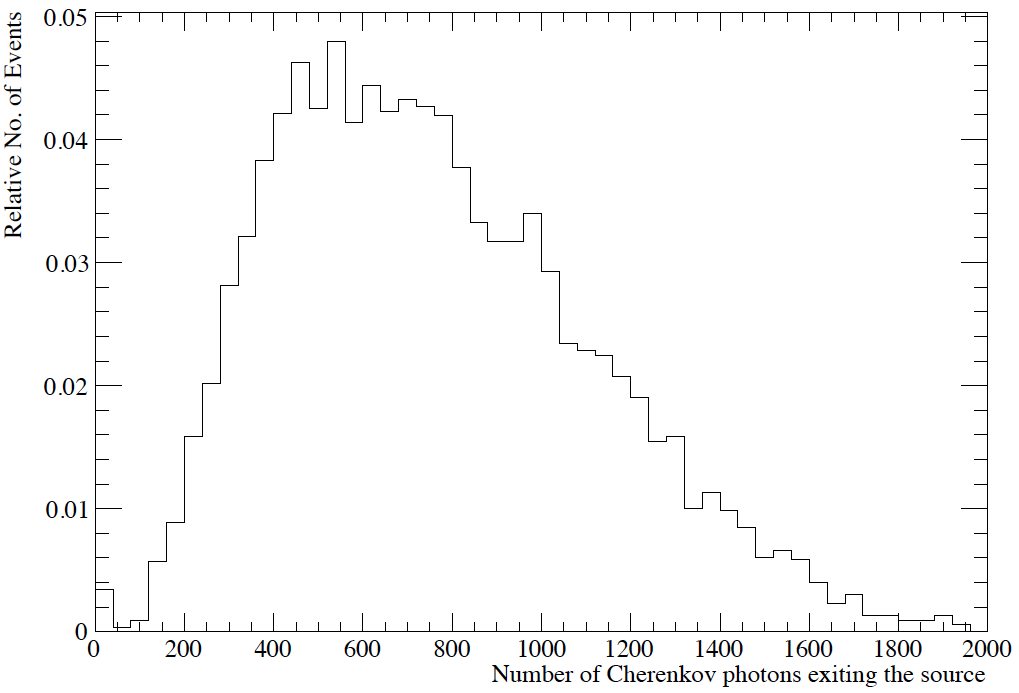
\includegraphics[width=.92\textwidth]{nhit.png}
   \caption{Distribution of number of Cherenkov photons exiting the source for events without scintillation light.}
   \label{fig:nphotons}
 \end{subfigure}
 \hspace{0.5cm}
 \begin{subfigure}{.48\textwidth}
   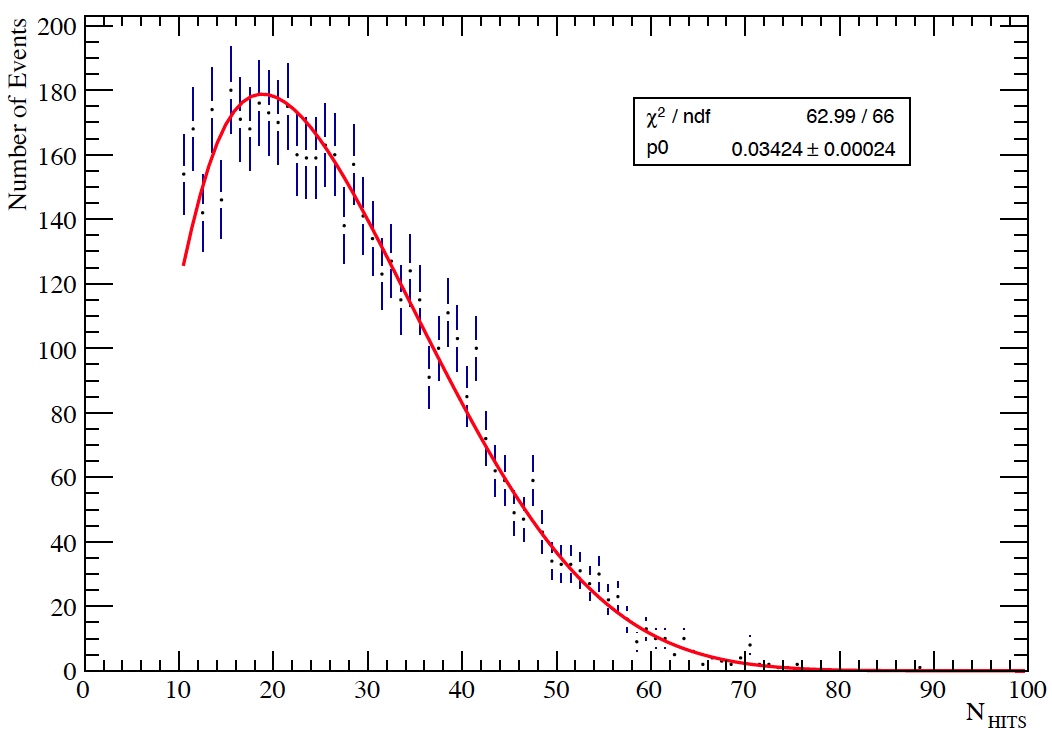
\includegraphics[width=.92\textwidth]{fit.png}
   \caption{Fit of NHit-distribution to sum of binomial distributions.}
   \label{fig:fit}
 \end{subfigure}
 \caption{Using RAT simulations of the Cherenkov source to extract the overall light collection efficiency. Figures taken from~\cite{Heintzelman:2013}. }
 \label{fig:heintzelman-plots}
 \end{figure}
 
\subsubsection{Cutting Bremsstrahlung Events}

\begin{figure}[]
\center{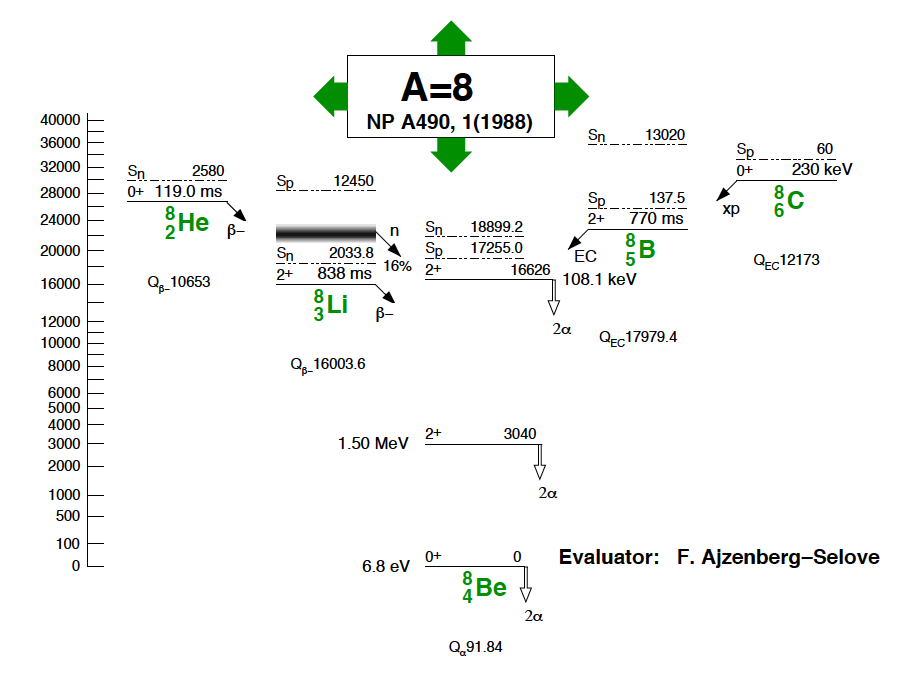
\includegraphics[width=.7\textwidth]{Ais8DecayScheme.png}}
\caption{\label{fig:decayscheme} A=8 decay scheme. Taken from~\cite{Tagg:2001}.}
\end{figure}
The decay of \Li in the Cherenkov source produces $\beta$s with an end-point energy of about 13\,MeV (see \Cref{fig:decayscheme} for the decay scheme). In addition to producing Cherenkov light in the acrylic, bremsstrahlung $\gamma s$ are also produced in a significant number of events.  These $\gamma s$  exit the source and are likely to Compton-scatter in the scintillator or water inside the AV.  Simulations indicate that Compton-scatter electrons are produced in about 1/3 of the events.  Although such events are not much different from non-bremsstrahlung events in either total light produced or PMT hit timing when the detector is filled with water, in scintillator fill they produce much more light and have a different timing profile.  In addition, their characteristics depend heavily on scintillator properties. It is therefore desirable to eliminate such bremsstrahlung events from the data-set. For this, a cut based on the likelihood ratio of the distribution of PMT hit-time residuals was found to be particularly effective. A time-only fitter, which uses the knowledge of the source position, was developed to do determine the event time from the event data.

\subsubsection{Extracting the light collection efficiency}
In order to monitor the light collection efficiency, the distribution of the number of photons exiting the Cherenkov
source per non-scintillation event are predicted by simulation, see Figure~\ref{fig:nphotons}. Then, the total probability of observing a certain number of hits is fitted to the NHit-distribution for simulated events, where the probability that a photon produces a hit is varied, see Figure~\ref{fig:fit}. This fit was performed for simulations with varying efficiencies and the extracted photon detection probabilities were found to change as expected.


\section{Design}
\label{chap:design}

See~\cite{wallig:2015} for the complete set of technical drawings for the Cherenkov source. We will be referring to pages inside this document in this section. 3D-rendered drawings are used in this section to identify the different parts of the source. For all detailed dimensions, please refer to~\cite{wallig:2015}.
\subsection{Cherenkov source}
The Cherenkov source consists of three main parts: the acrylic decay chamber and the PMT assembly inside the neck (newly designed and constructed) and the steel housing inherited from the SNO \Li source. See Figures~\ref{fig:design-1} and~\ref{fig:design-2}.
\begin{figure}
\center{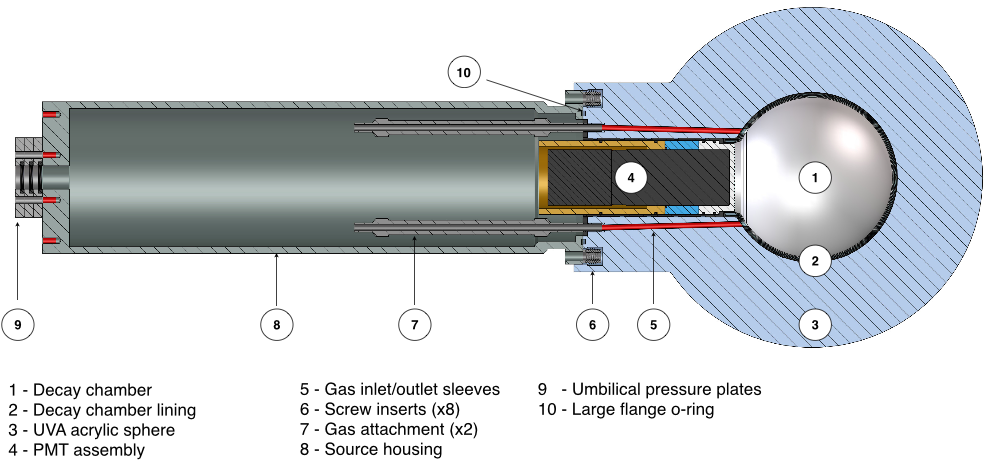
\includegraphics[width=1.0\textwidth]
{Design-1.png}}
\caption{\label{fig:design-1}Schematic of the fully assembled Cherenkov source.}
\end{figure}
\begin{figure}
\center{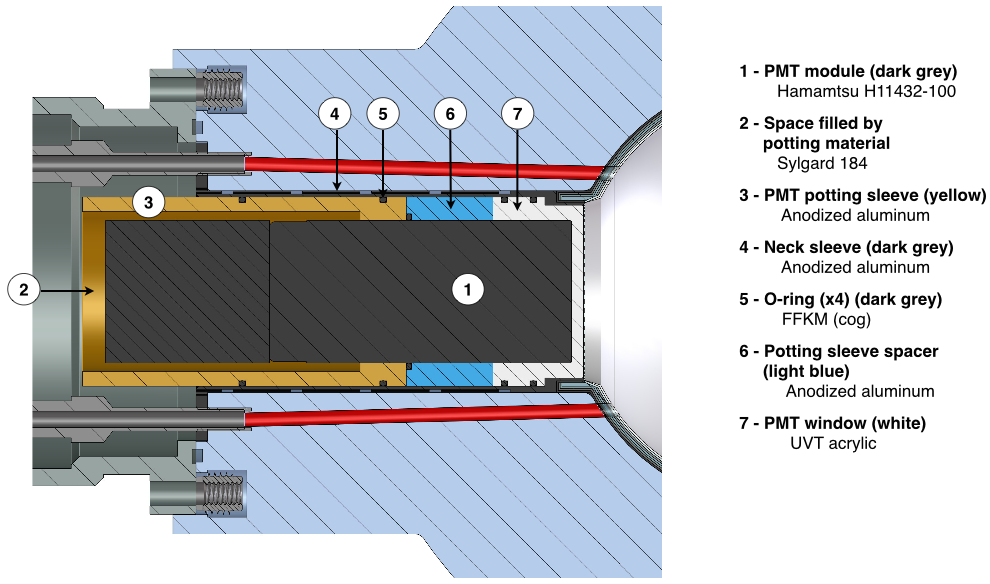
\includegraphics[width=1.0\textwidth]
{Design-2.png}}
\caption{\label{fig:design-2}Detail of the PMT assembly.}
\end{figure}

\subsubsection{Decay chamber}
The decay chamber consists of the following parts and materials:
\begin{itemize}
    \item {\bf Acrylic sphere}: The sphere is made out of UVA acrylic, supplied by RPT (Reynolds Polymer Technology). Details of the construction of the sphere can be found in Section~\ref{chap:construction}.   
    \item {\bf Weld-on\,\#40}: The two halves of the the sphere are bonded using Weld-on\,\#40. Details on the cement testing and bonding procedures can be found in Section~\ref{sec:bond}.
    \item {\bf Decay chamber lining}: The inside of the decay chamber is lined with an opaque, reflective and wavelength-shifting coating, which consists of 4 layers of paint. The first three layers are black paint. The last layer is a reflective white paint that has TPB mixed in. For details on the application and testing of the decay chamber lining see Sections~\ref{sec:lining} and~\ref{sec:liningtest}.
    \item {\bf Neck sleeve}: A thin neck-sleeve made from anodized aluminum is potted in place using Sylgard 184 after the first two layers of the black paint have been deposited. It serves to ensure light-tightness, specifically around the PMT window. The shape at the top of the sleeve is such that a canal is created between the acrylic neck and the neck sleeve, see Figure~\ref{fig:design-2}. This canal is filled up with paint in the subsequent paint-stages. See also \cite{wallig:2015}, page 14.
    \item {\bf Gas inlet/outlet sleeves}: Two thin steel capillaries are potted inside the gas inlet and outlets holes with Sylgard~184. These are needed in order to ensure light-tightness and do not form gas seals. The inlet lines are threaded into the acrylic and the threads are potted in with Sylgard~184. 
    \item {\bf Screw inserts}: The attachement of the decay chamber to the steel housing is done by way of 8 stainless steel screws. 8 screw-inserts are glued in place inside the top of the decay chamber using Weld-on\,\#40. See \cite{wallig:2015}, page 14.
    \item {\bf Large flange o-ring}: A single large o-ring is placed in the plane where the steel housing is connected to the decay chamber. It is made from FFKM material, see Section~\ref{sec:oring}.
\end{itemize}
\subsubsection{PMT assembly}
\begin{itemize}
    \item {\bf Tag PMT}: The PMT module fits inside the neck to observe the scintillation light inside the decay chamber. The module is a Hamamatsu H11432-100 which has an integrated high voltage supply that requires only low voltage (+5V) to operate.
    \item {\bf Potting sleeve}: Made from anodized aluminum (\cite{wallig:2015}, page 8). The PMT is potted inside the potting sleeve using Sylgard~184. 
    \item {\bf Potting sleeve spacer}: Made from anodized aluminum (\cite{wallig:2015}, page 9). Needed to bridge the space between the potting sleeve and the PMT window.
    \item {\bf PMT window}: Made from UVT acrylic (\cite{wallig:2015}, page 10).
    \item {\bf Small neck o-rings}: There are 4 small o-rings between the PMT assembly and the neck-sleeve, they are made from FFKM material. See Section~\ref{sec:oring} for a discussion on the FFKM o-rings.
\end{itemize}
\subsubsection{FFKM o-rings}
\label{sec:oring}
The o-rings inside the flange and the neck are custom-made Resist-RS80AL/FFKM 80 black o-ring produced by COG (C. Otto Gehrckens GmbH \& Co. KG). This type of o-ring was tested for compatibility with LAB, see~\cite{snoplus:2013}. An additional test using LAB-PPO was done in 2015 and shows a slight deviation from the control sample (see Figure~\ref{fig:FFKM}). The FFKM material is preferred over the less compatible FKM.
\begin{figure}
\center{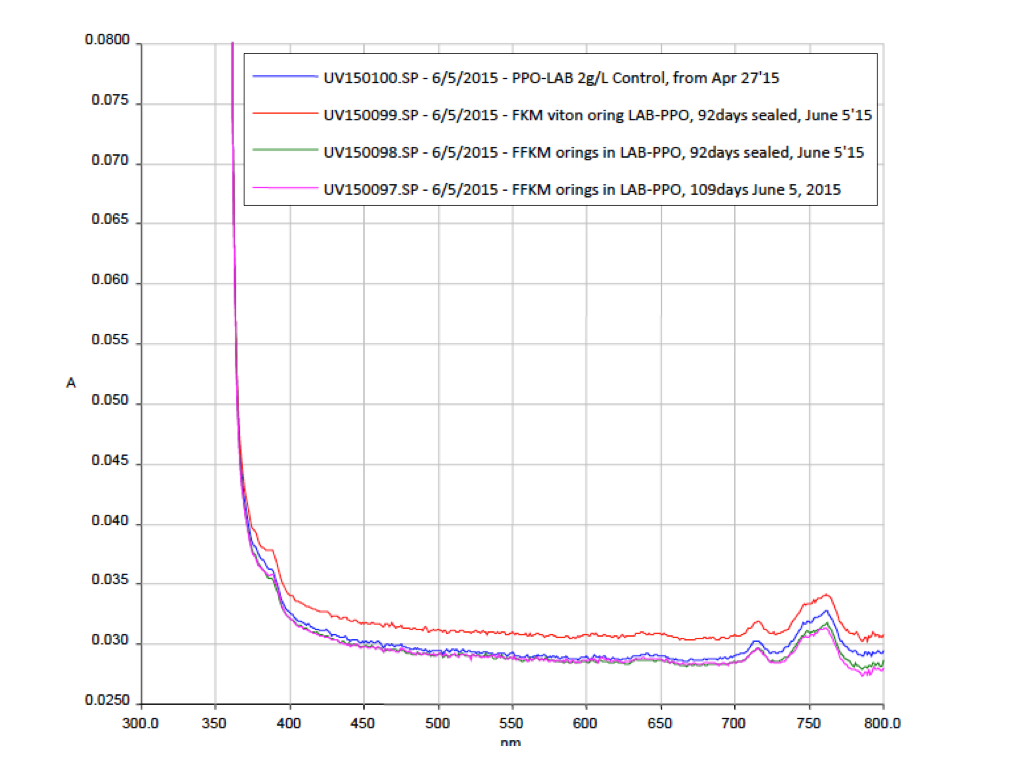
\includegraphics[width=0.7\textwidth]
{FFKM.png}}
\caption{\label{fig:FFKM}Detail of the FFKM compatibility test result. From ~\cite{snoplus:2013}.}
\end{figure}
\subsubsection{Sylgard 184}
\label{sec:sylgard}
The potting material used is Sylgard~184 manufactured by DOW Corning Silicones. It is a two-component silicone encapsulate (not room temperature vulcanization) which dries to a medium durometer (hardness) rubber. It will allow the parts to expand and contract without over-constraint. It is used at four locations in the Cherenkov source:
\begin{itemize}
    \item PMT into PMT-sleeve: used to pot the back-end of the PMT inside the PMT holder. This will protect the HV circuit and hold the PMT in place.
    \item Neck-sleeve: used to hold the neck sleeve (anodized aluminum) in place.
    \item Gas inlet tube: used to hold the steel capillary in place.
    \item Gas outlet tube: same as above.
\end{itemize}
In normal operation mode, the potting material does not come into contact with the scintillator. The material was tested and was found to be incompatible with LAB-PPO, see Section~\ref{sec:comptest}. The material swells when in contact with LAB-PPO and there was a change in absorbance.
\subsubsection{Steel housing}
The housing (\cite{wallig:2015}, page 12) and the gas connections (\cite{wallig:2015}, page 13) are inherited from the SNO \Li source. The housing is made of stainless steel and can be shortened if needed. One way to handle different types of connections is to add a flange when shortening the steel housing, a suggested implementation of this flange is shown in Figure~\ref{fig:flange}. The gas connections can also be changed if needed. The housing will be polished and cleaned before the final assembly and deployment of the source.

\begin{figure}
\center{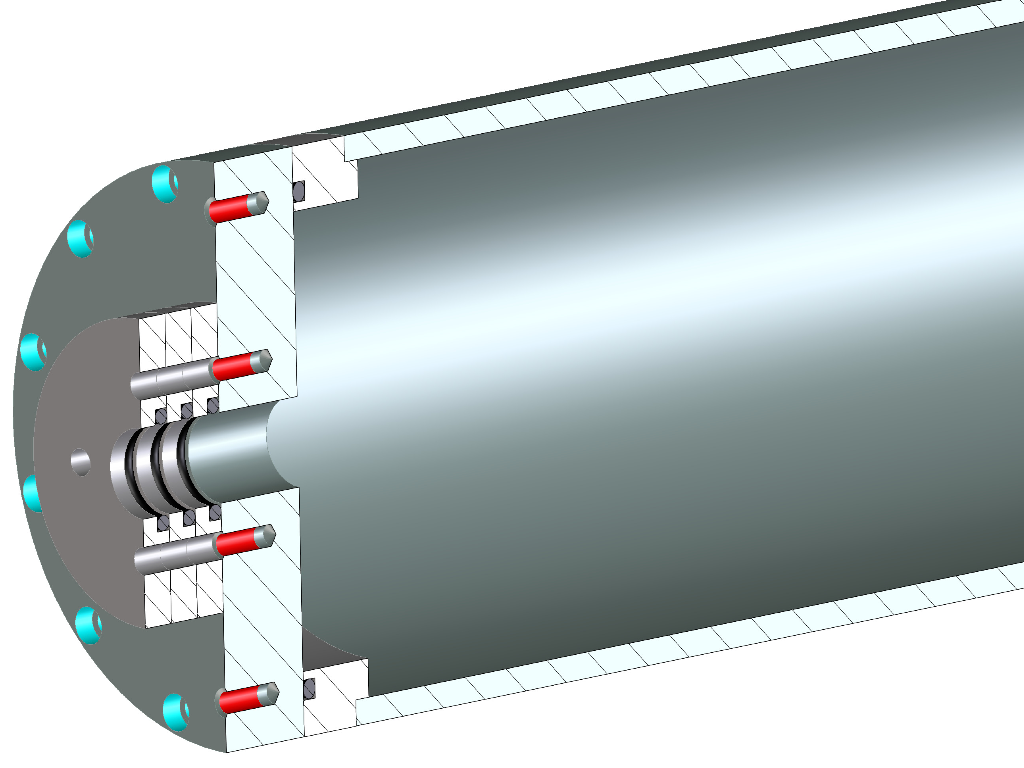
\includegraphics[width=.5\textwidth]
{flange.png}}
\caption{\label{fig:flange} Schematic of a suggested flange to be welded at the top of the source housing. }
\end{figure}

\subsection{Deployment hardware}
This section discusses the interface of the source with the SNO+ deployment hardware. 
\subsubsection{Umbilical and connection}
For deployment during the SNO+ water-phase, the SNO \Li umbilical will be re-used. Figure~\ref{fig:sno_umbilical} shows the cross-section of this umbilical. It contains the required gas-transport lines in addition to the electrical wires; one for the PMT signal and three for the low-voltage for the PMT (ground, power, control voltage). The umbilical currently has no connector. Just as was done for SNO, the plan is to connect the gas hoses and wiring for the PMT by hand while the top of the source (steel housing) is exposed. Then the sealing pressure plates (Figure~\ref{fig:pressureplates}) are slid down and bolted together. The so-called 'lighthouse' attachment, see Figure~\ref{fig:connection}, sits on the endcap and is used to attach the source to the weight (if needed) and the manipulator carriage.

\begin{figure}
\begin{subfigure}{.57\textwidth}
\center{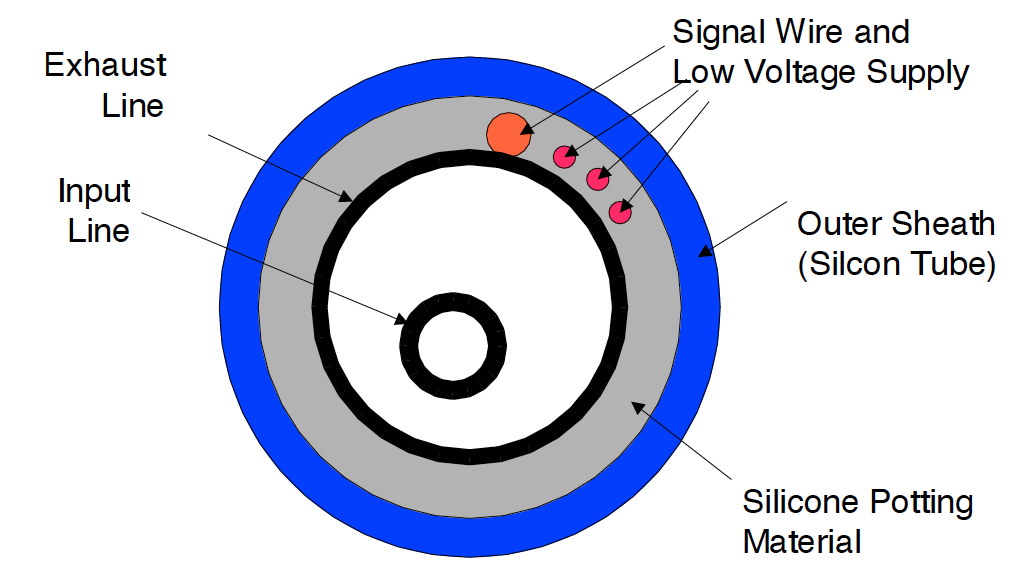
\includegraphics[width=1.0\textwidth]
{8Li-Umbilical.png}}
\caption{\label{fig:sno_umbilical} The SNO \Li umbilical cross-section. Taken from~\cite{Tagg:2001}.}
\end{subfigure}
\hspace{0.5cm}
\begin{subfigure}{.35\textwidth}
  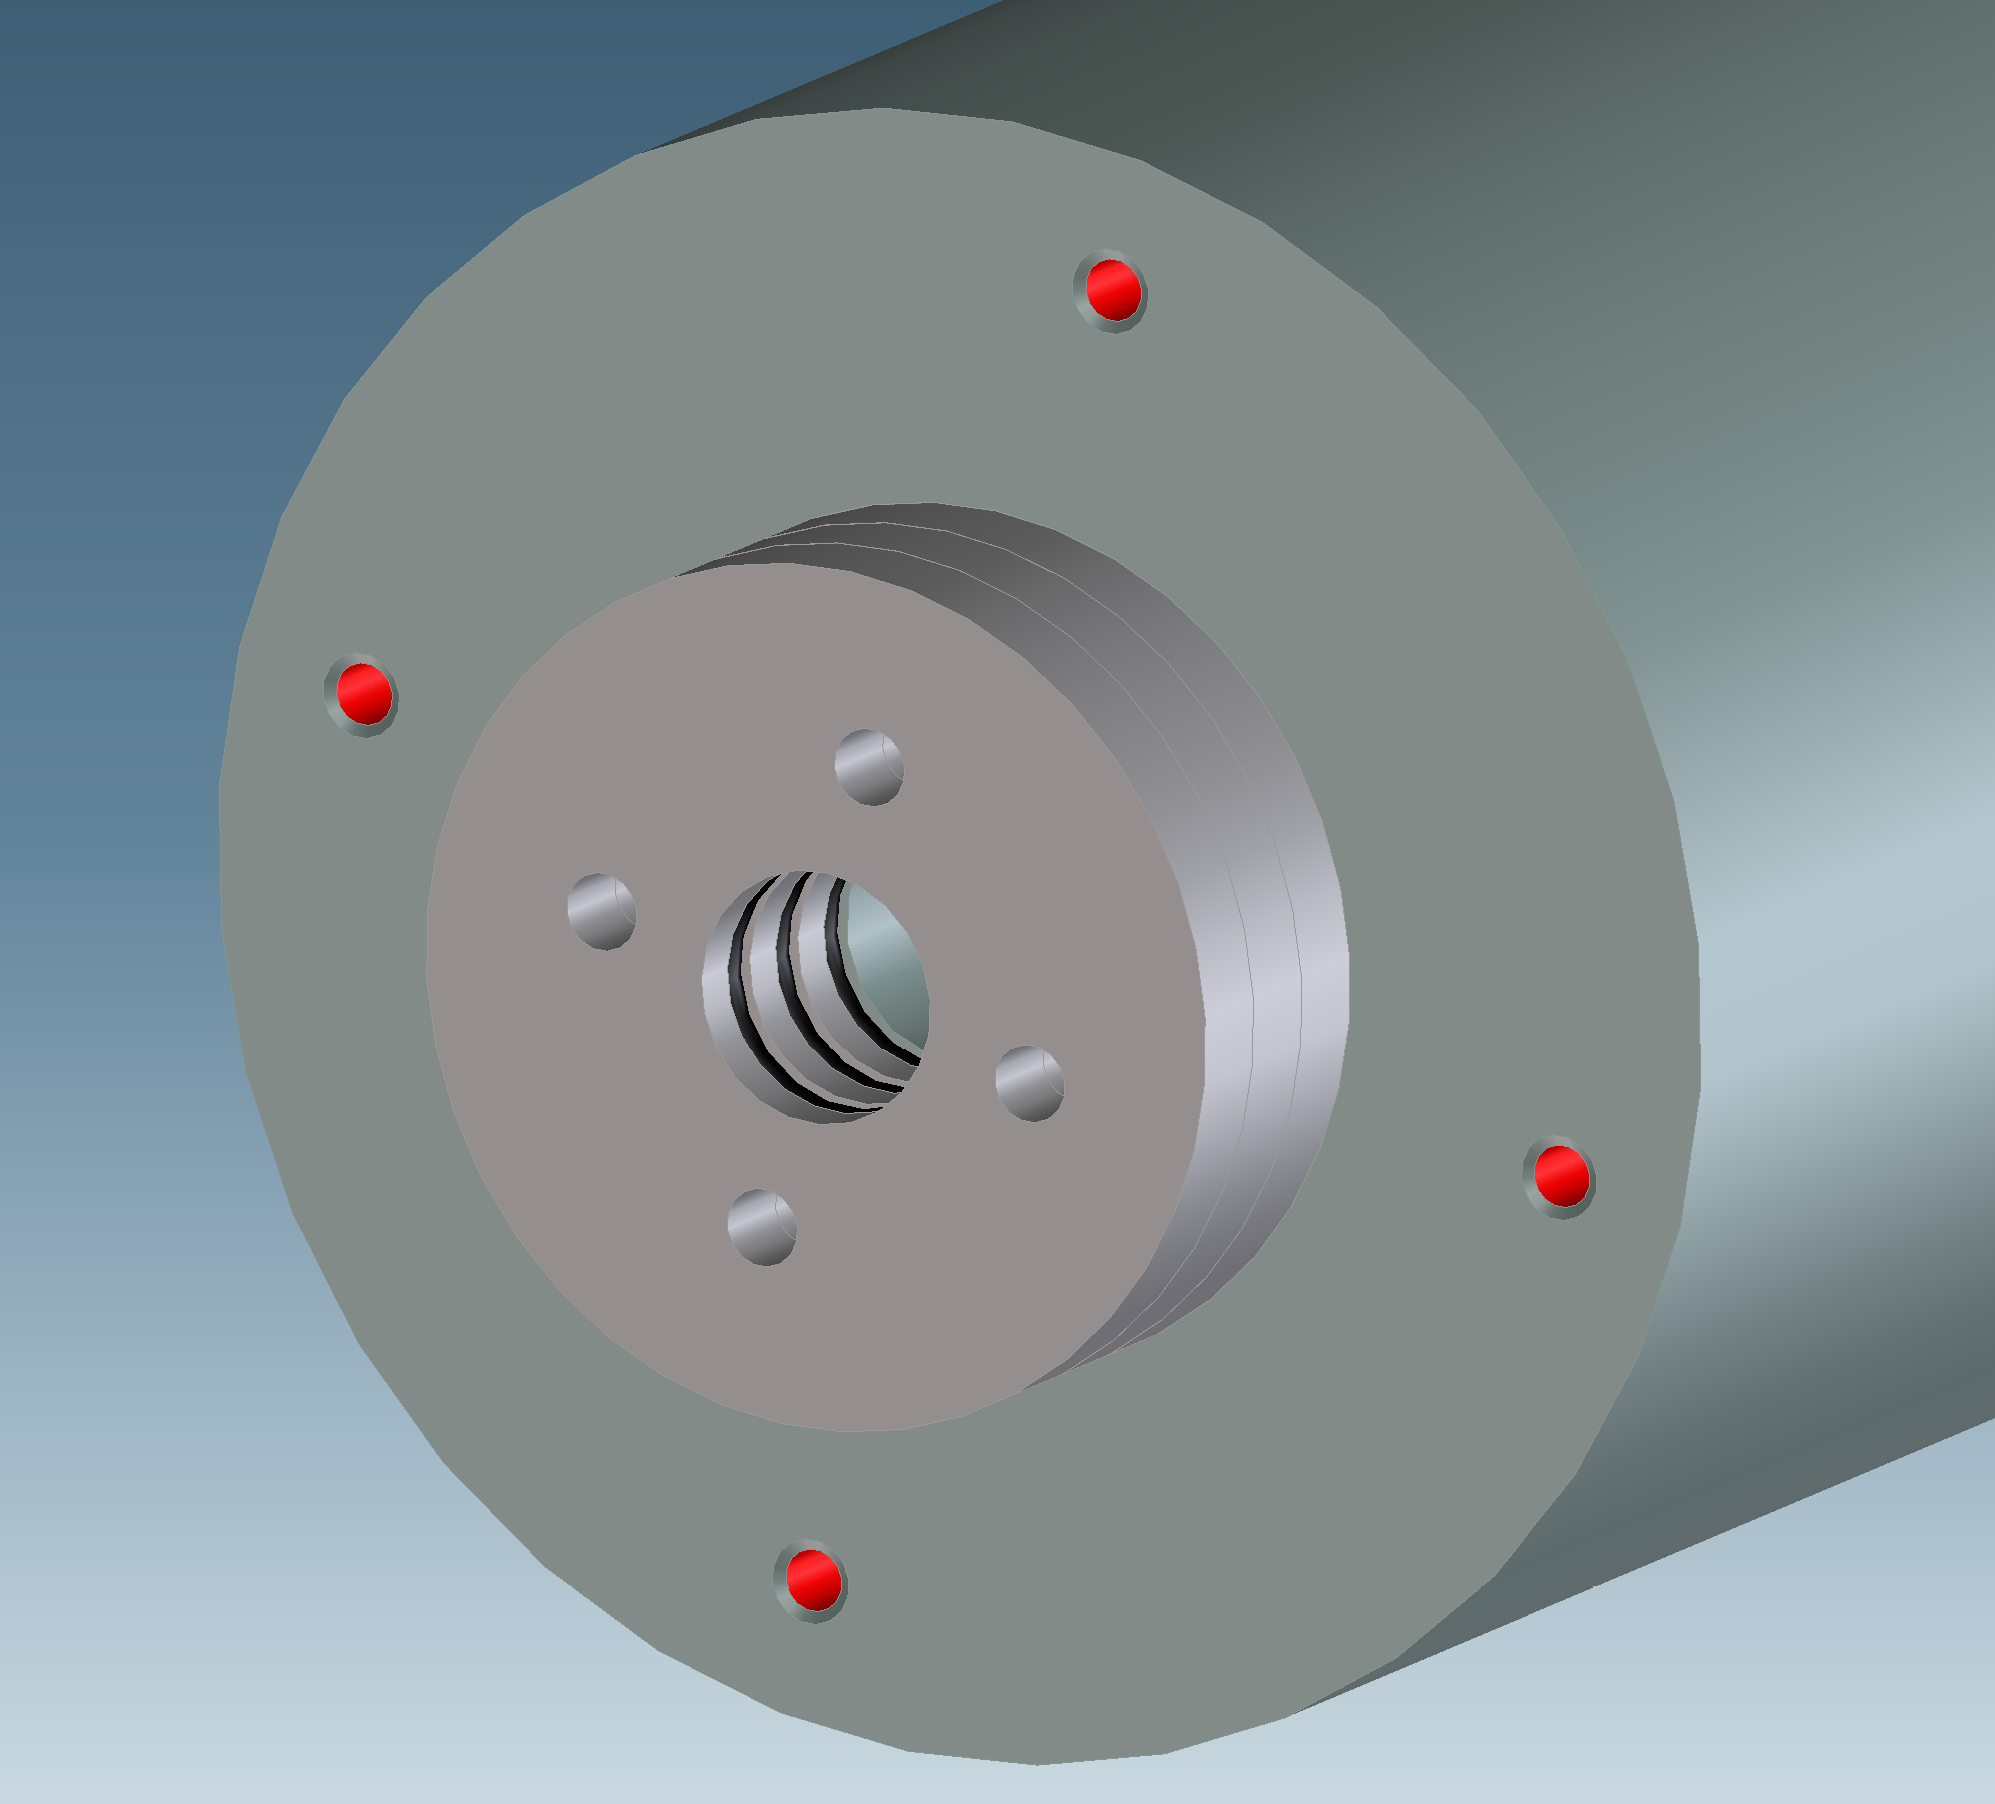
\includegraphics[width=\textwidth]{HousingTop.png}
  \caption{\label{fig:pressureplates} The sealing pressure plates.}
\end{subfigure}
\caption{Details of the umbilical and the water-phase umbilical connection to the source housing.}
\end{figure}

\begin{figure}
\center{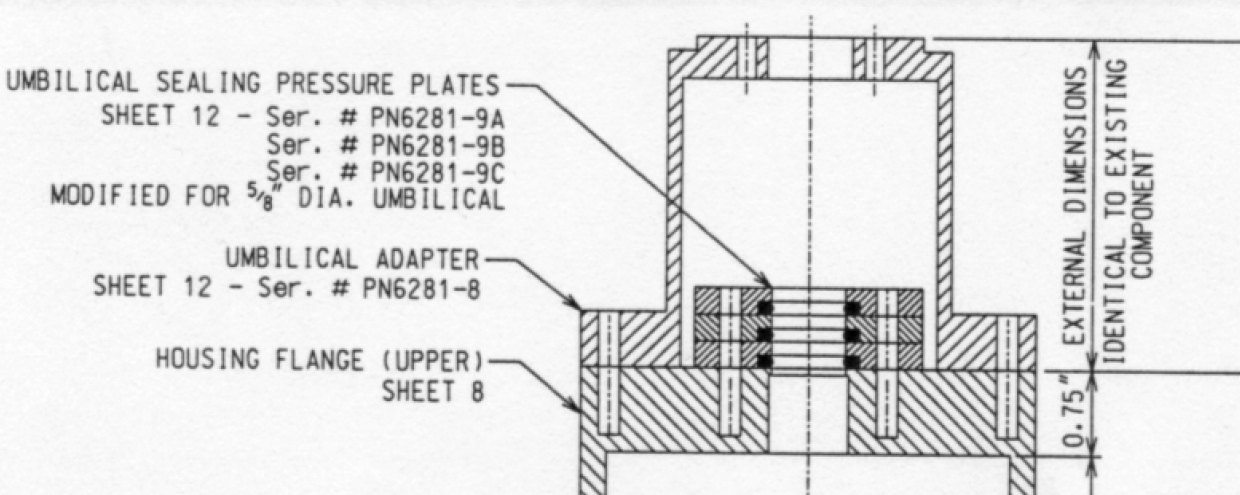
\includegraphics[width=.8\textwidth]
{UmbilicalConnection.png}}
\caption{\label{fig:connection}Detail of the SNO \Li technical drawing, showing the top assembly with the pressure plates and the 'lighthouse'. Taken from~\cite{Tagg:2001}.}
\end{figure}

The umbilical that will be used for deployment in the liquid scintillator still needs to be produced. It is expected to be of a similar design as the SNO \Li umbilical with the difference that there will be a source connector permanently attached to the umbilical. An adapter needs to be designed to connect to the Cherenkov source. 
\subsubsection{Source storage box}
The storage box for the liquid scintillator phase is currently under design. It is being designed as tall as possible and the current height is estimated at 70\,cm. It is recommended that there is at least 10\,cm clearance for the sources.
\subsection{Weight and length estimates}
The source is very buoyant. The weights of the current source (with the original steel housing) were calculated in water and LAB-PPO. The weight can be changed by adding weights or by removing part of the steel housing. The weight in air is estimated to be 15.3\,kg. The deployed weight is 3.77\,kg in UPW and 5.34\,kg in LAB. In addition, the weights in particular failure-modes were also calculated. See Table~\ref{tab:weights} for the details of the expected weight in these situations.
The source can be shortened by cutting the steel housing. This can be done quickly and on short notice. For water phase deployment the source was shortened to minimum length in order to meet weight requirements for the deployment system. 

\begin{table}[h!]
\centering
\begin{tabular}{|l|l|l|l|l|} \hline
                & UPW (air)     & UPW (depl.)   & LAB (air)     & LAB (depl.)   \\ \hline
No breach       & 15.23         & 3.77              & 15.23         & 5.34              \\ \hline
Leak in
decay chamber   & 16.13         & 4.67              & 16.00         & 6.12              \\ \hline
Leak in
housing         & 17.89         & 6.43              & 17.52         & 7.64              \\ \hline
Leak in
both          & 18.79         & 7.33              & 18.30         & 8.41              \\ \hline
\end{tabular}
\caption{\label{tab:weights} Cherenkov source weight, all weights are in kilograms}
\end{table}

\section{Decay chamber construction}
\label{chap:construction}

\subsection{Overview}
The Cherenkov source decay chamber is a hollow acrylic sphere. It is formed out of two acrylic slabs that are bonded together. The annealing, bonding, decay chamber lining and PMT potting are described in the next sections. The bonding, painting and storage of the decay chamber was done inside a class-1000 clean room at LBNL.
The construction of the Cherenkov source decay chamber has roughly the following steps:
\begin{enumerate}
    \item Pre-anneal: the acrylic is pre-annealed at the production site (RPT).
    \item Machine cycle 1 (see~\cite{wallig:2015}, page 2): hollow out the decay chamber and neck from the two slabs. Machine holes for alignment pins. 
    \item Polish: the inside of the decay chamber is polished using NOVUS heavy and fine scratch remover (Diatomaceous earth/Silica)~\cite{polish}. 
    \item Sand: the bond-plane is sanded to prepare for the bond using NORTON Blue-Bak waterproof paper (Silicon carbide) grit, 220, 320, 400, 600~\cite{sand}.
    \item Ultra high vacuum cleaning.
    \item Anneal: the two machined slabs are annealed.
    \item Ultra high vacuum cleaning.
    \item Mask: masking paint (Micro Mask MI-7~\cite{masking}) is used to protect the inside of the decay chamber from the cement. This product is easily removed with water.
    \item Bonding: bond the two halves together using Weld-on \#40, an acrylic cement. 
    \item Remove masking: once the cement has set, remove the masking from the inside of the decay chamber.
    \item Machine cycle 2 (see~\cite{wallig:2015}, pages 5 and 6): remove excess acrylic to form sphere, drill the gas inlet/outlet holes, machine o-ring groove.
    \item Ultra high vacuum cleaning.
    \item Decay chamber lining: use paints and TPB to line the inside of the decay chamber. This also requires potting of the neck sleeve and gas inlet and outlet sleeves.
    \item PMT potting: pot the tag PMT inside the PMT sleeve.
    \item Assembly and testing.
\end{enumerate}

\subsection{Annealing}
Before bonding, the blocks must be annealed to remove any residual stresses. The annealing process raises the temperature of the acrylic in a controlled way so that stress frozen into the cold solid acrylic can relax away, and then lowers the temperature in a controlled way so that new stress is not developed. This is necessary to ensure that there are no residual stresses that will cause reduced optical clarity (crazing) or mechanical failure (poor bond). The blocks were placed in an annealing oven shown in Figure~\ref{fig:oven} that was programmed to follow an annealing curve containing an initial ramp, a soak phase, and a cool-down ramp. Most information for acrylic annealing was obtained from an Air Force / Navy acrylic fabrication specification MIL-P-6997B(ASG) and the Handbook of Acrylics. The thickness of the acrylic during annealing is 152\,mm which is used for calculating the lengths of the annealing stages, and a soak temperature of 80\degree C was chosen to ensure the acrylic can relax without risking deformation of the machined surfaces. The final annealing curve is shown in Figure~\ref{fig:annealing}.

\begin{figure}
\begin{subfigure}{.54\textwidth}
  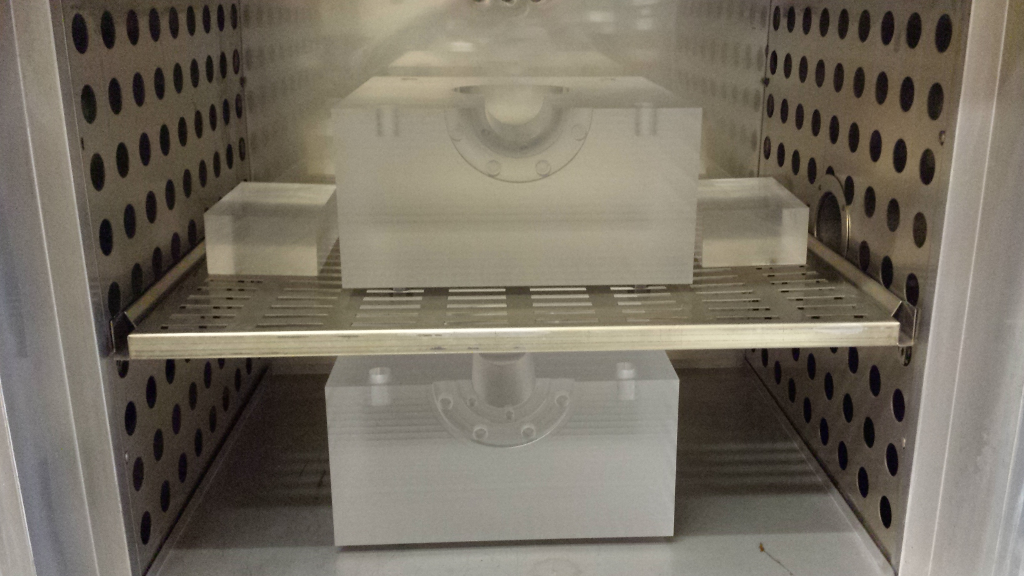
\includegraphics[width=\textwidth]{annealing_oven.png}
  \caption{Source and reference-block acrylic in oven.}
  \label{fig:oven}
\end{subfigure}
\begin{subfigure}{.47\textwidth}
  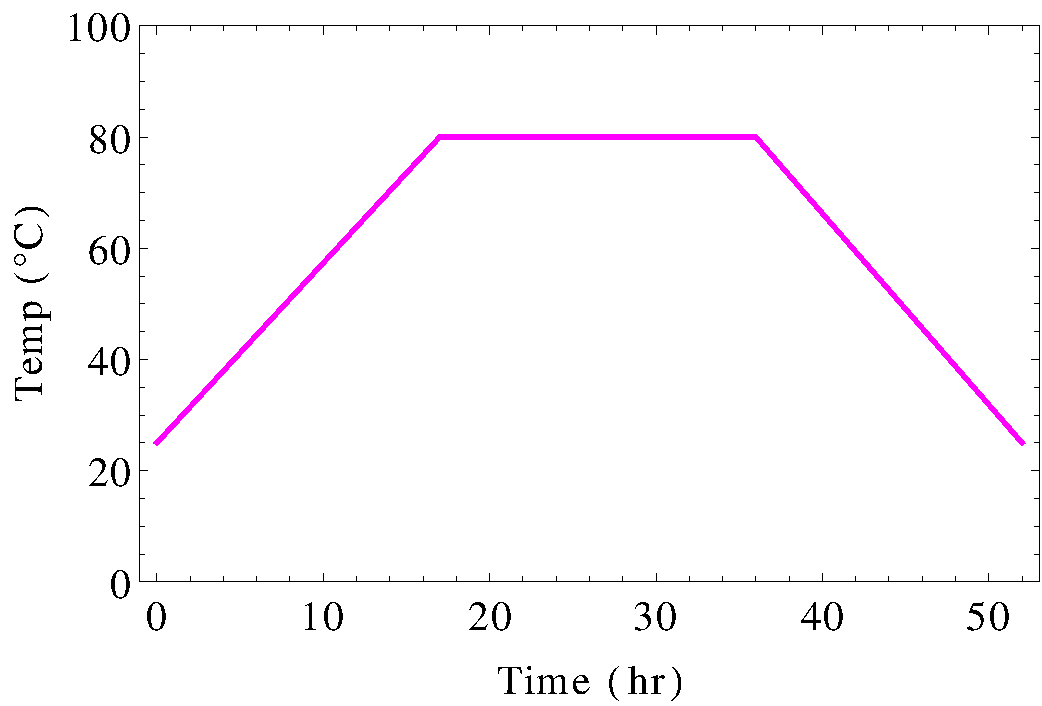
\includegraphics[width=\textwidth]{annealing_curve}
  \caption{51 hour annealing cycle.}
  \label{fig:annealing}
\end{subfigure}
\caption{Acrylic must be annealed to allow any residual stresses that may result in optical flaws post-bonding to relax away.}
\label{fig:annealfig}
\end{figure}

\subsubsection{Initial Ramp}
An initial ramp from room temperature to soak temperature is necessary for very thick acrylic to avoid large temperature gradients that may deform the acrylic or introduce more stress. Data for this consideration was obtained from~\cite{anneal} which is summarized in Figure~\ref{fig:ramp}. The available data did not go up to the 152\,mm thickness, but a clear linear trend allowed for extrapolation.

\subsubsection{Soak Phase}
After the acrylic has reached a uniform annealing temperature the stress must have time to relax away. This soak time depends on the magnitude of the residual stress present and the thickness of the acrylic. Data~\cite{anneal} for this stage is in Figure~\ref{fig:soak}. Again, available data did not go up to 152\,mm thickness, and although a clear linear trend was not evident, extrapolation with a linear trend would seem to be an overestimate and only give additional time for relaxation.

\subsubsection{Cool-down Ramp}
A slow cool-down is necessary to avoid large thermal gradients that will induce new stress in the acrylic. The rate of cool-down is dependent on the thickness of the acrylic, and data gathered on this is summarized in Figure~\ref{fig:cooldown}.  Once again, available data~\cite{anneal} did not go up to 152\,mm thickness but there is a clear exponential trend that was extrapolated.

\begin{figure}
\begin{subfigure}{.32\textwidth}
  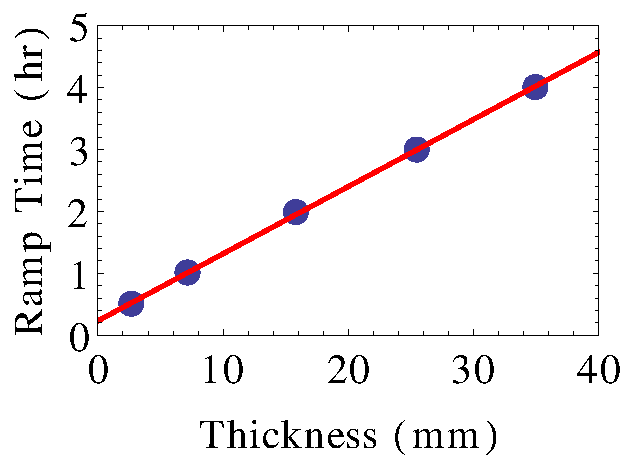
\includegraphics[width=\textwidth]{annealing_ramp}
  \caption{Ramp length}
  \label{fig:ramp}
\end{subfigure}
\begin{subfigure}{.32\textwidth}
  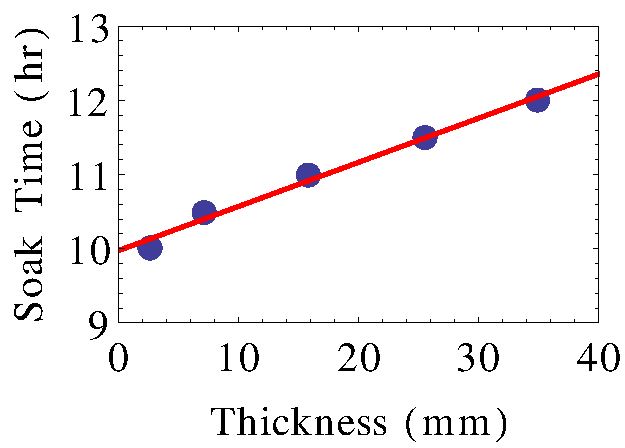
\includegraphics[width=\textwidth]{annealing_soak}
  \caption{Soak time}
  \label{fig:soak}
\end{subfigure}
\begin{subfigure}{.32\textwidth}
  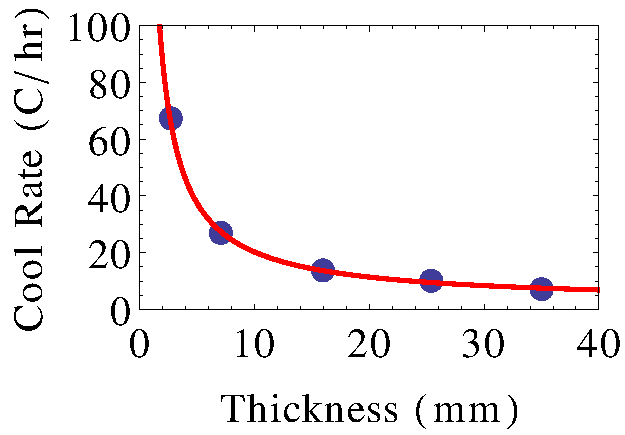
\includegraphics[width=\textwidth]{annealing_cooldown}
  \caption{Cooling rate}
  \label{fig:cooldown}
\end{subfigure}
\caption{Data~\cite{anneal} used in extrapolating annealing curve parameters for $80^{\circ}$ C annealing.}
\label{fig:annealdata}
\end{figure}

\subsection{Bonding of the acrylic decay chamber}
\label{sec:bond}
The bond of the two acrylic slabs is required to be optically flawless, strong and leak-proof. A substantial amount of tests were done to ensure that these properties could be achieved for the final bond. This section discusses the choice of bonding agent and the bonding procedures.
\subsubsection{Testing of the bonding agent}
In order to test the different bonding agents, a series of glue tests have been conducted (Figure~\ref{gluesetup1}. Details are described in~\cite{tanner:2014}. For these tests, two pieces of acrylic are bonded together using different bonding agents. Once the bond has cured, a piece of PVC pipe is sealed to the top of the acrylic, directly above the glue bond. The PVC pipe is approximately half-filled with LAB-PPO scintillator. A collector dish is sealed directly under the acrylic to collect potential leaking. If the LAB-PPO leaks through the bond, it will be collected by the glass container below the acrylic. A UV lamp, emitting at 254\,nm, is used to see the leakage since LAB-PPO scintillates under this wavelength light. Any small leak can be clearly determined by shining the UV lamp (Figure~\ref{gluesetup2}). Both UV transparent (UVT) and UV absorbent (UVA) acrylic are tested in this setup.

\begin{figure}[t!]
    \centering
\begin{subfigure}{.45\textwidth}
    \centering
  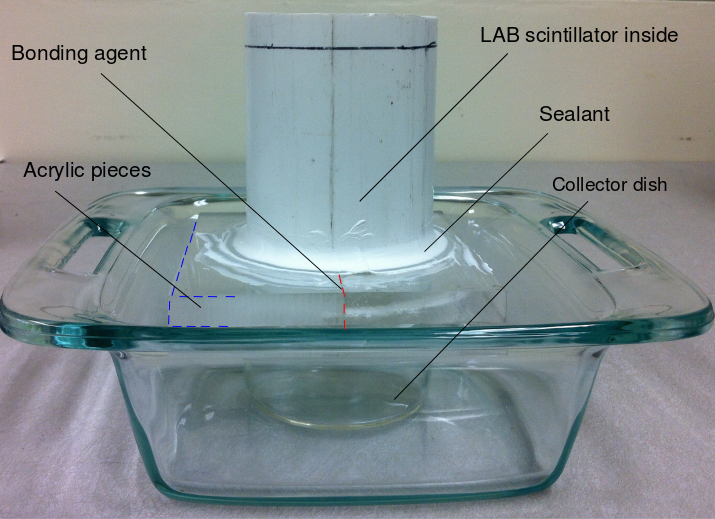
\includegraphics[height=2in]{setup_2.png}
  \caption{Overview of the setup to determine if the bonding agent leaks LAB-PPO over an extended period of time.}
  \label{gluesetup1}
\end{subfigure}
\hspace{0.5cm}
\begin{subfigure}{.45\textwidth}
    \centering
  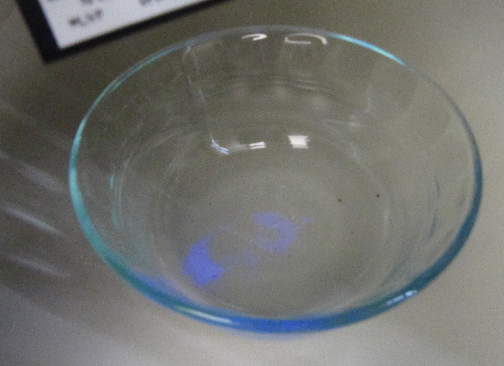
\includegraphics[height=2in]{SmallLeak.png}
  \caption{Method to determine leaking. One drop of LAB-PPO has been sitting in this glass container for over three months and it still clearly scintillates under UV exposure.}
  \label{gluesetup2}
\end{subfigure}
  \caption{The bonding test setup.}
\label{fig:gluesetups}
\end{figure}


Three different types of bonding agents have been tested with the small table-top setups: methylene chloride, Acrifix 2R 0190, and Weld-on\,\#40. The methylene chloride chemically bonds the two pieces of acrylic together. Both the Acrifix 2R 0190 and the Weld-on\,\#40 need to be mixed with a catalyst and are acrylic cements. They both contain methylene chloride and have pot lives of about 20 minutes. The length of time for the adhesive to become a solid, the cure time, for Acrifix and Weld-On is 60 minutes and 20 minutes, respectively.

Four setups have been closely monitored for leaking and are presented in Table~\ref{tb:glues}. The setups are created from two pieces of acrylic, each measuring 5.7$\times$5.7$\times$1.905\,cm for the UVT and 5.7$\times$5.7$\times$2.54\,cm for the UVA. These pieces were cut from the sample acrylic sent from Reynolds, and the difference in thickness are due to the dimensions of the supplied samples. The acrylic is the exact same type as those which that be used to make the source. The two pieces are bonded along one of the long sides, giving a glue bond either 1.905 or 2.540\,cm thick. This is significantly less thick than the thickness of the source (6\,cm) which ensures that we have a conservative measurement of the ability of the glue to prevent leaking.  It was found that, in case of the UVA, the methylene chloride setup leaked. This could be because of small air-bubbles that are trapped inside the bond-plane. 
\begin{table}
  \begin{center} %centers the table on the page
    \begin{tabular}{ | c | c | c | c | c | c  |} 
        \hline 
Setup \# & Glue Type & Acrylic Type & Leaked & Dates \\ \hline 
5 & Methylene Chloride  & UVT & No & 5/1/13 - Present  \\ 
6 & Methylene Chloride  & UVA & Yes & 5/16/13 - 5/28/13  \\ 
7 & Acrifix   & UVT &  No & 5/1/13 - Present  \\ 
8 & Weld-On\,\#40 & UVA & No & 5/31/13 - Present  \\ 

    \hline
    \end{tabular}
    \end{center}
        \caption{An overview of the different leak-test setups and their results.}
    \label{tb:glues} 
\end{table}

\subsubsection{Cement Decision}
Weld-On\,\#40 was chosen as the bonding agent, because of the clear advantages over methylene chloride in the leak tests and the familiarity within SNO+ (not present for the Acrifix products). Weld-On\,\#40 has shown to be leak resistant, durable, and easy to use. Additionally, a Weld-On\,\#40 bond maintains good optical properties, is very strong at room temperature and the slow cure is expected to produce less stress in the acrylic after the bond.
\subsubsection{Bonding procedure}
\label{chap:bondproc}
The bonding of the two acrylic blocks that make up the Cherenkov source decay chamber is a critical step in the Cherenkov source construction. The procedure for this bonding was developed after many tests and mock-bonding walk-throughs. The bonding procedure describes how to safely and cleanly prepare and apply the bonding agent, how to align and clamp the two acrylic pieces together and how to deal with the excess cement that will leak inside the decay chamber. A few general notes should be made first. 
\begin{itemize}
    \item The Weld-On\,\#40 curing time depends on the amount of component B mixed into component A. For a while after the bond has been made, the bond plane will appear a bit cloudy since the Weld-On has not started curing yet. Once the curing starts, the bond-plane will become invisible.
    \item Do not machine the gas inlet and outlet in the first machining phase. This would make the masking of the decay-chamber much harder and one would risk filling up the holes with Weld-On\,\#40.
\end{itemize}

The detailed bonding procedures are described here. 
\begin{enumerate}
\item Clean up and clear the workspace.  
\item Assemble all equipment and make sure everything is there. Anything that will touch the Weld-On\,\#40 or the blocks will need to be UHV cleaned. The following is needed:
\begin{itemize}
\item UHV cleaned cups, Teflon stirring stick, clamps (for source and reference piece), razor blades and long tweezers.
\item UHV cleaned flat screwdriver which can be used to pry the two block apart in case of a serious issue with the bond.
\item Machined and UHV cleaned acrylic blocks, with the decay chamber polished and the bond-plane sanded. All inside surfaces should have been masked and the masking has been verified to be completely dry. The positions of the clamps need to be marked on the top block.
\item UHV cleaned acrylic alignment pins in contrasting color.
\item UHV cleaned reference UVA acrylic blocks.
\item Cleaned precision scale.
\item Fresh Weld-On\,\#40, components A and B. Make sure to inspect the color of the Weld-On\,\#40, it should not be yellow. 
\item New syringe to add component B to A.
\item Vacuum pump system.
\item Valve system for compressed air. This includes a filter for the compressed air-line.
\item Flashlight to inspect bond-plane.
\item Reference blocks.
\item Camera in place and taking pictures.
\item Smaller camera for close-up shots.
\item Pen and clean-room paper for notes.
\item Weld-On\,\#40 suction system. This will be used to suck the excess Weld-On\,\#40 out of the decay chamber before it has time to cure. 
\end{itemize}
\item Unpack everything, position on table.
\item Position the two acrylic blocks in the correct position on the table. One should be lying on its back, with the alignment pins in place. The other block should be standing on its side in such a way that rotation will be minimal when joining the two blocks.
\item Inspect the bond-surface. Remove any clear debris with clean-room wipe. 
\item Inspect the inside edges of the bond-plane and remove any masking from the bond-plane using the edge of a razor. Any masking that remains would be locked inside the bond-plane. 
\item Carefully open the Weld-On\,\#40 away from the two acrylic blocks. The opening  might release some spray droplets that could fall on the blocks. Be aware that a strong odor will be present once the Weld-On\,\#40 is opened. 
\item Using a precision scale mix exactly 5 parts in 100 grams of the Weld-On\,\#40 catalyst (component ``B'') with the Weld-On\,\#40 glue (component ``A'') at room temperature. Component ``B'' should be added slowly and over the entire surface area of component ``A'' to prevent initial hardening of the glue. Stir very thoroughly with a Teflon stick until the mixture is completely mixed. We used 200 grams of component A and a more shallow mixing cup.
\item Immediately after stirring, place the mixture in a vacuum chamber to remove air bubbles from the mixture. The pressure should be reduced to at least 10 Torr. The air bubbles in the mixture rise to the top and begin the mixture will seem to froth. At this point the pressure should be released and the air bubbles will pop and begin to disappear. This process should be repeated at least three times, or until the air bubbles are almost completely gone.
\item Pour the glue on one piece.  A few cm thick layer, closer to the decay chamber edge than to the outside of the blocks. About 1\,cm away from edge. Follow the line of the decay chamber edge. Do not worry about cement leaking over the edges. The blue masking will remove the cement left on the inside of the source and the outside of the source will be machined again. The more cement there is on the masking, the harder it is to remove it.
\item Bond the acrylic pieces. Two people lift the  top block together while the third person stands on the side to guide the correct positioning of the pins compared to the top block. Make sure that the blocks are oriented correctly. Fit the top piece on top of bottom piece using the guidance pins.
\item Quickly use the flashlight to inspect the glue plane. There are a few seconds where the blocks could still be pulled apart if a large contamination is spotted in time. Use the flat screw-driver to do so if needed.
\item Clamp the acrylic pieces together. Start by adding the middle clamp. Make sure that the clamp is oriented away from the neck-opening. Then, add the corner clamps. Their position is marked by red dots on the top block. Check with flashlight for bubbles while clamping is happening. Do not over-clamp.
\item Using a suction-system, suck out as much Weld-On\,\#40 out of the decay chamber as possible. This will make the removing of the masking much easier
\item In order to ensure the glue dries,  blow compressed air into the decay chamber while it is clamped. This will push the vapor from the Weld-On\,\#40 out of the decay chamber and allow the glue to dry properly. Do not let the compressed air line touch the blocks.
\item Bond the reference blocks and clamp with metal clamp.
\item Once the glue is dried (about 1 hour), remove the masking. Test the texture of the outside glue-blobs to make sure the glue has hardened. Using some sort of tweezers/grabbers, peel the masking off from the inside of the source. Twisting technique.
\item Let the glue cure for minimum 48 hours.
\item Inspect the source to make sure that all masking is gone. If needed, put it through the UHV shop before the next machine cycle.
\end{enumerate}

Once the final machining cycle is done, the source is ready for the application of the decay chamber lining.

\subsection{Decay chamber lining}
\label{sec:lining}
The hard UV helium scintillation light of the alphas inside the decay chamber is used to tag events with the internal neck PMT. This light must not escape the decay chamber as this would be hard to model and would pollute the dataset with additional non-Cherenkov light. Therefore the lining of the decay chamber must be made opaque while the top layer should be reflective enough to ensure sufficient photons reach the PMT. This surface should also wavelength shift the hard UV light to more visible wavelengths detectable by the PMT. Finally, since the electrons that produce Cherenkov light must travel through this surface, the thickness should be minimal and the effect on the electrons should be easy to model. To accomplish these goals, three thin layers of black paint are deposited for opacity followed by a layer of white paint mixed with TPB for reflectivity and wavelength shifting. In small scale tests this was found to produce a nominally uniform, thin, and opaque surface.

\subsubsection{Preparation and procedure} 
To ensure the source meets cleanliness requirements and that unwanted materials did not get trapped in the paint, this entire process was carried out in a class-1000 clean room. The method for applying the paint was to pour the paint mixture into the neck with the neck facing up, rotate the source by hand to coat the inside of the decay chamber, place the source neck down on a drying stand that blows filtered air into the decay chamber while allowing excess paint to drip down out of the neck, and finally cut away any excess paint that dripped out the neck with a scalpel (see Figure \ref{fig:drying}). The mass of the source was measured before paint was added and after excess was cut away for each layer which was used later to infer layer thickness. To ensure light tightness of the source, the gas inlet and outlet tubes were fitted with stainless steel capillaries that protrude into the decay chamber enough to allow the paint layers to form a light tight seal. To prevent these capillaries from filling with paint a Teflon rod is inserted that extends past the capillary into the decay chamber and remains for the entire painting process. The aluminum neck sleeve that receives the PMT and ensures light tightness of the neck region was added during the opaque paint layers.

\begin{figure}
\begin{subfigure}{.28\textwidth}
  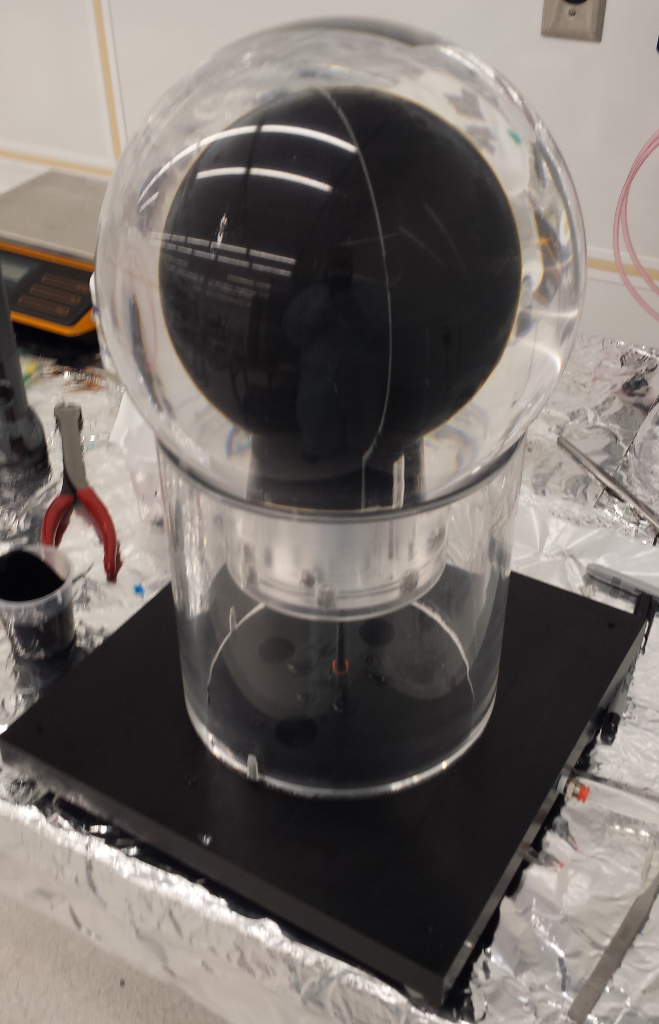
\includegraphics[width=\textwidth]{drying_stand.png}
  \caption{Test source drying on the drying stand.}
\end{subfigure}
\hspace{0.5cm}
\begin{subfigure}{.67\textwidth}
  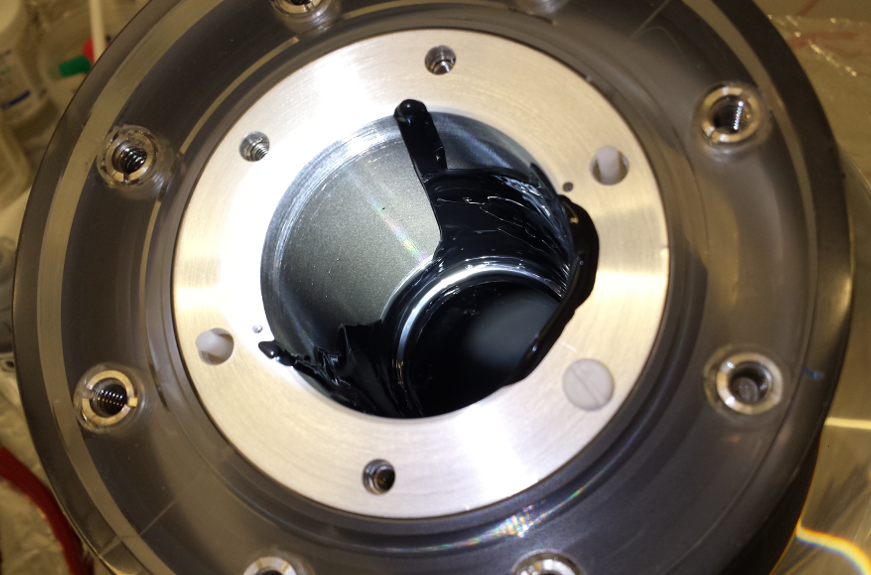
\includegraphics[width=\textwidth]{paint_drips.png}
  \caption{After drying the final black layer, the minimal excess paint dripping is cut away from the aluminum neck sleeve by a scalpel.}
\end{subfigure}
\caption{The painting and drying setup was tested with the test source in a class 1000 clean room at LBNL. Note that the neck sleeve used here for the test source was not anodized whereas the final source will have a black anodized aluminum neck sleeve.}
\label{fig:drying}
\end{figure}

\subsubsection{Opaque paint deposition}
The black paint used here was Golden Fluid Acrylics carbon black which had a consistency suitable for direct application to the decay chamber and was tested for light tightness and surface quality at smaller scales, see also~\cite{tanner:2014}. Each layer used 60\,mL of paint of which some fraction dripped out. For the first two of three layers a Teflon sleeve similar to the aluminum neck sleeve was inserted into the neck to prevent black paint from adhering to the neck region while allowing excess paint to drip out. Using a removable Teflon sleeve for the first two layers enhanced the uniformity of the paint thickness near the neck by preventing pooling (see Figure \ref{fig:minisource_paint}) that would occur if the aluminum neck sleeve were present. Prior to the third layer of black paint, the aluminum neck sleeve that accepts the PMT assembly was potted into the neck using Sylgard 184, a silicone encapsulate, allowing the third layer of black paint to fill any gaps around the neck sleeve to decay chamber interface resulting in a light tight seal. The encapsulate was applied to the outside of the neck sleeve and inserted into the source with the neck facing down to ensure no encapsulate dripped into the decay chamber. After the encapsulate cured on the drying stand, the final layer of black was applied.

\subsubsection{Reflective paint + TPB deposition}
This final layer was a mixture of 40\,mL of deionized water, 20\,mL of Vallejo white paint, and 5\,g of TPB. The addition of deionized water made the mixture approximately the same consistency as the black paint, and upon drying the remaining layer is mostly TPB crystals with a white paint binding that adheres well to the black paint surface. 5\,g of TPB using this deposition method was shown to give approximately the same scintillation brightness as the SNO \Li source when illuminated under a UV lamp. Further testing of the wavelength-shifting efficiency and reflectivity of this top layer is necessary since they directly affect the tagging efficiency. Other deposition methods either resulted in a very non-uniform layer, or, in the case of toluene evaporation deposition, dissolved the paint and acrylic in small scale tests.

\begin{figure}
\begin{subfigure}{.35\textwidth}
  \centering
  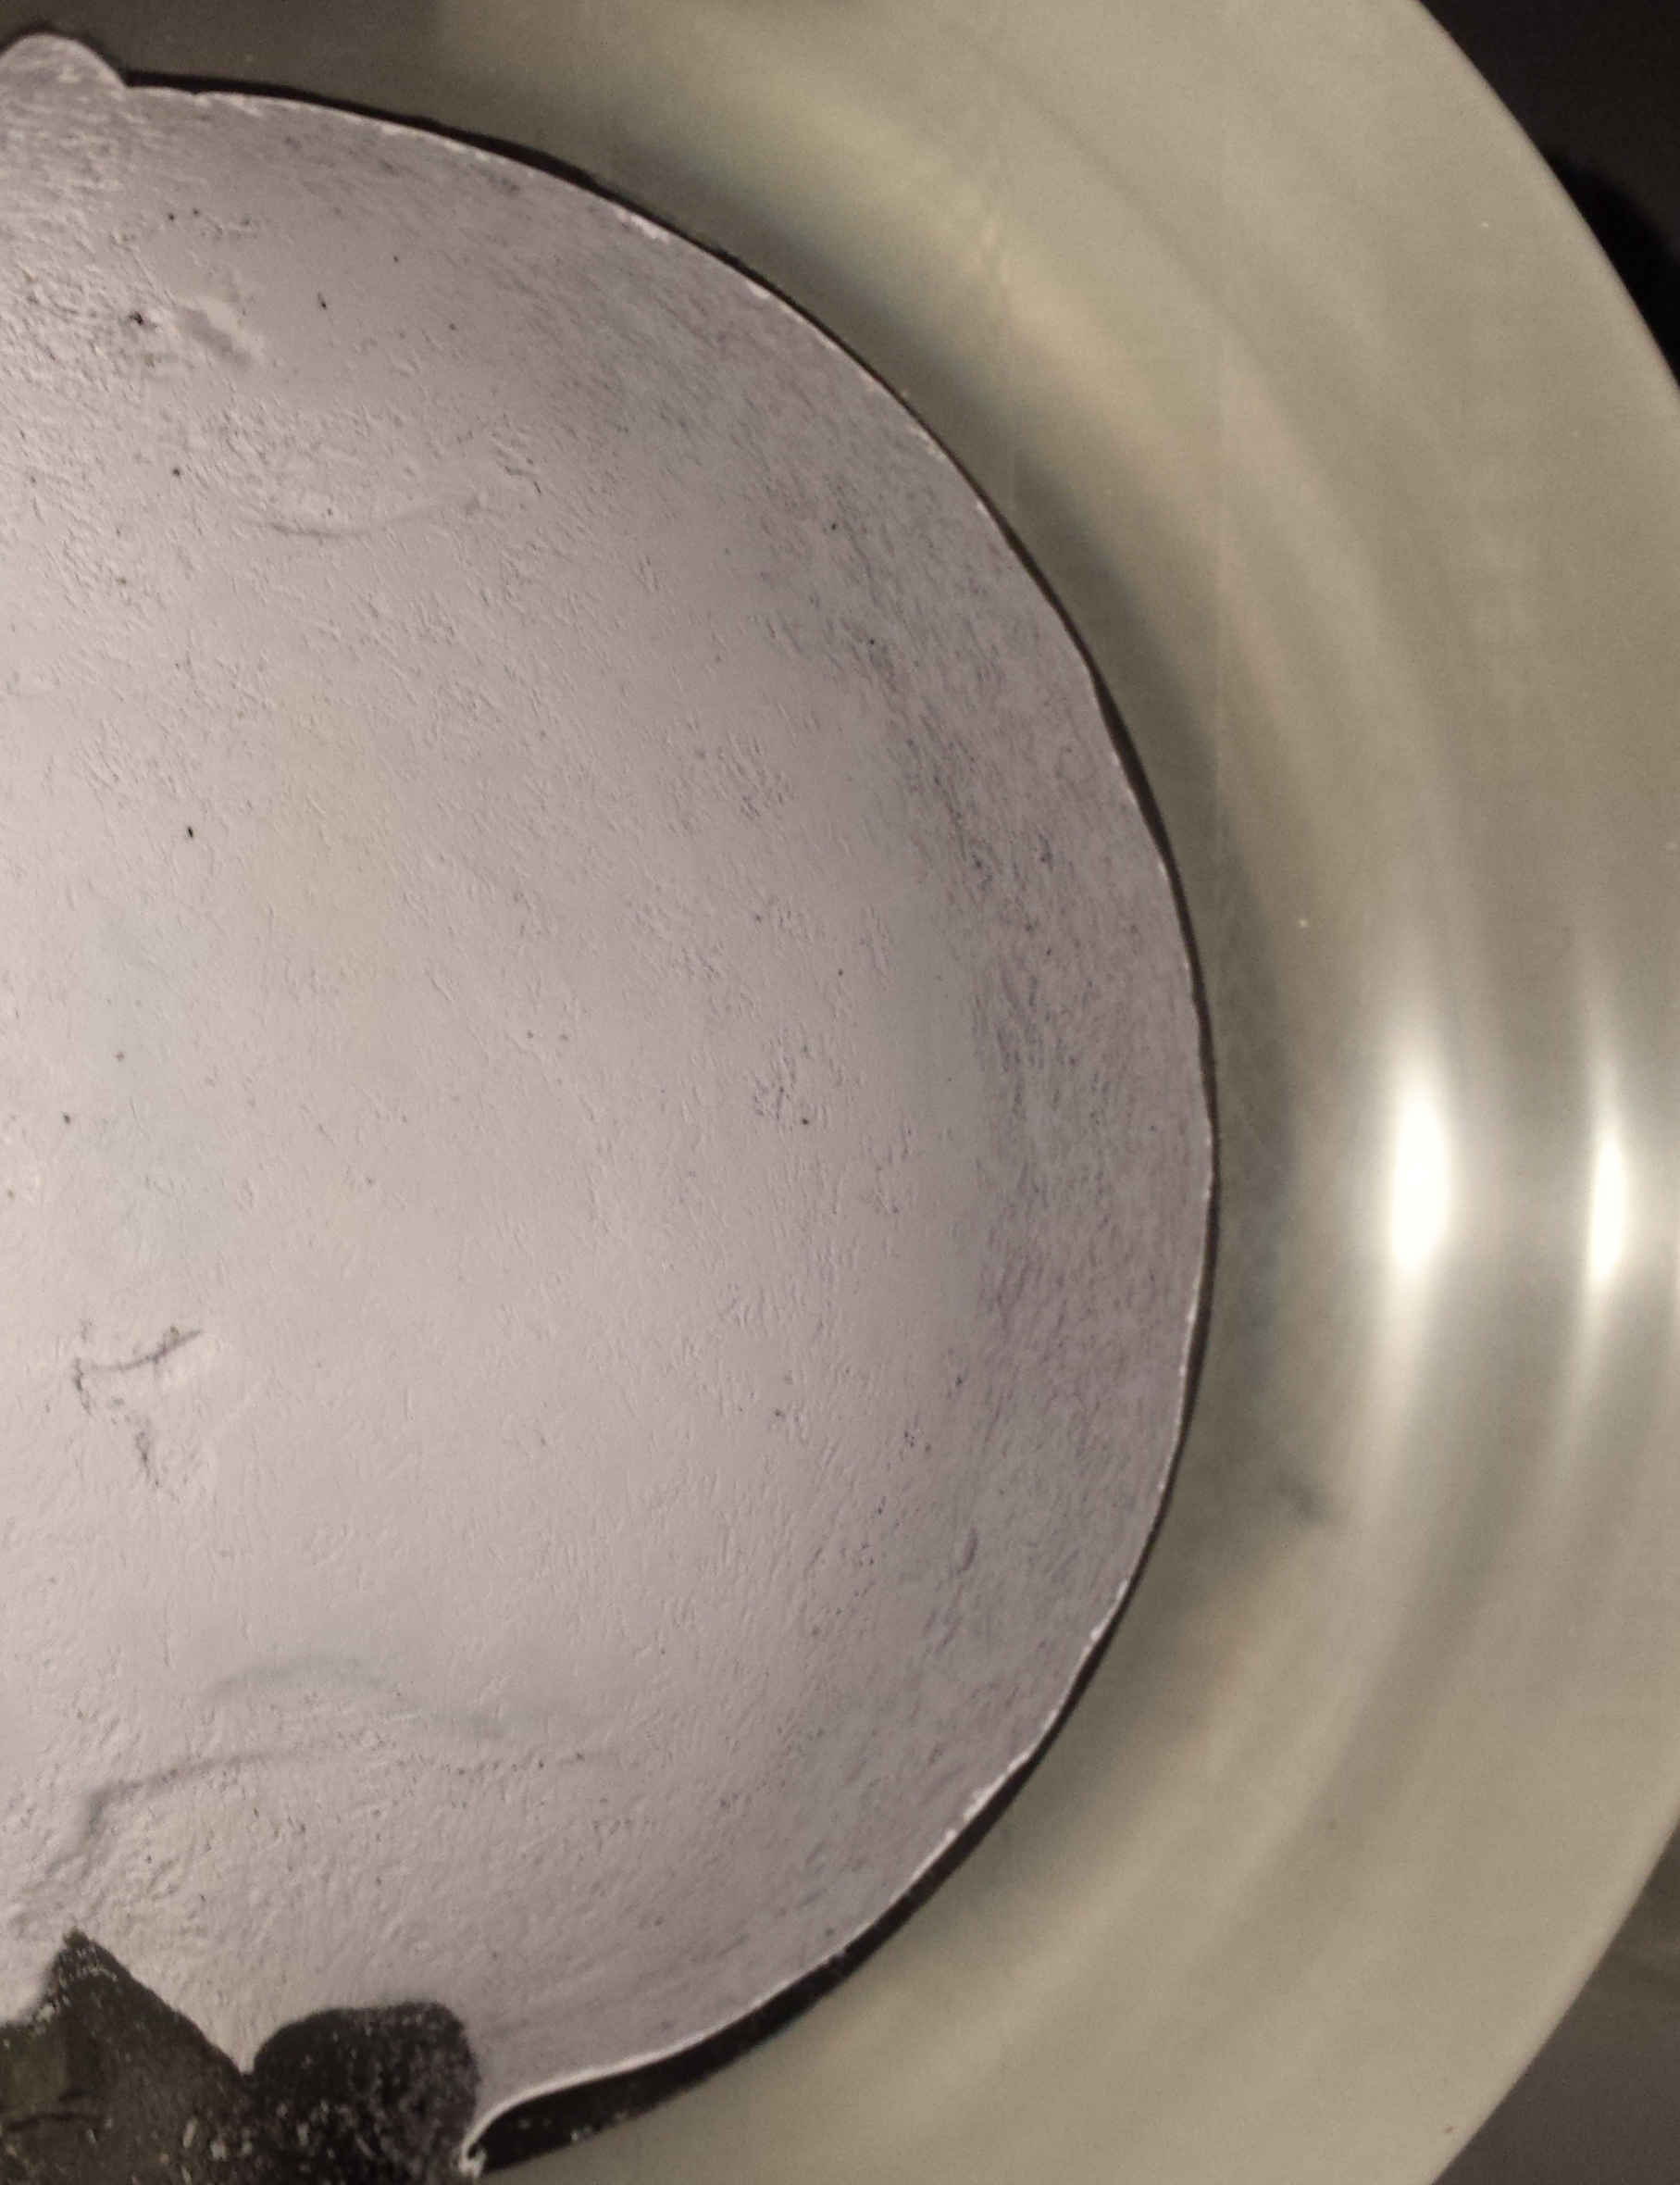
\includegraphics[width=0.8\textwidth]{minisource_paint.png}
  \caption{Small scale painting test showing cross-section of paint thickness. The pooling near the bottom was reduced by allowing easier drainage of paint for the first two layers, resulting in less anisotropy than pictured here.}
  \label{fig:minisource_paint}
\end{subfigure}
\hspace{0.5cm}
\begin{subfigure}{.55\textwidth}
  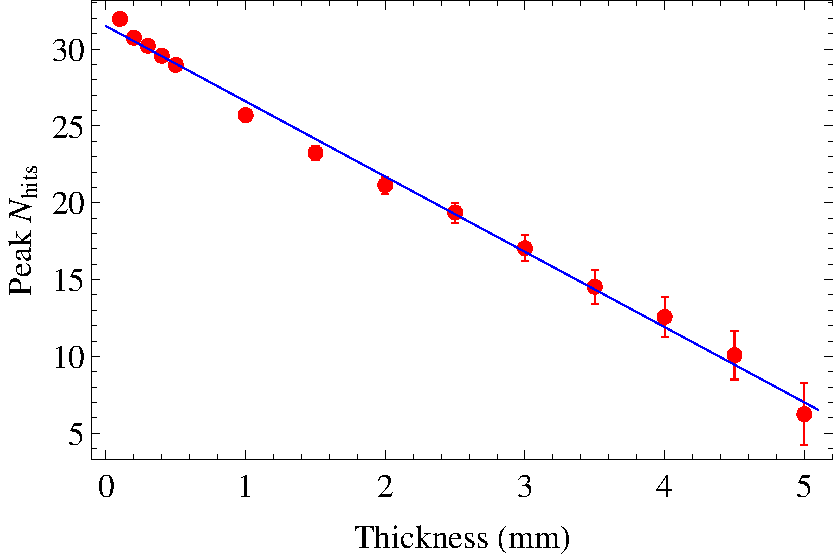
\includegraphics[width=\textwidth]{100k_realistic_nonoise_hits_vs_thickness}
  \caption{Simulation in scintillator phase SNO+ of \Li beta decays inside decay chamber volume with various smooth and isotropic paint layer thicknesses. As expected this follows a roughly linear trend representing the energy loss of the electrons in the paint.}
  \label{fig:meannhits}
\end{subfigure}
\caption{Small scale painting results and preliminary simulations of NHit response for \Li beta decays for various paint thicknesses assuming the simplest case of a smooth paint layer.}
\label{fig:prelimpaint}
\end{figure}

\subsubsection{Surface quality and thickness}
After each layer the surface was visually inspected to ensure no major flaws or clumps were found. Smaller scale tests indicated that the paint layers will be thicker near the neck than opposite the neck due to the drying orientation (anisotropy), that the mean paint thickness would be around 1\,mm, and that 10\% variations in thickness (roughness) are to be expected (Figure~\ref{fig:minisource_paint}). The roughness is expected to vary with a characteristic length scale of approximately 1\,cm according to the cross section of the small scale paint test.

To explore the effects of mean thickness and surface roughness on NHits, simulations of \Li electrons were done using a source geometry in RAT and various different paint layers. Simulations with perfectly smooth paint layers indicated that a 0.1\,mm change in mean paint thickness is conservatively a 5\% change in mean NHits (Figure~\ref{fig:meannhits}), so it will be necessary to know the thickness of the paint very well. 

\begin{figure}[h!]
\begin{subfigure}{.53\textwidth}
  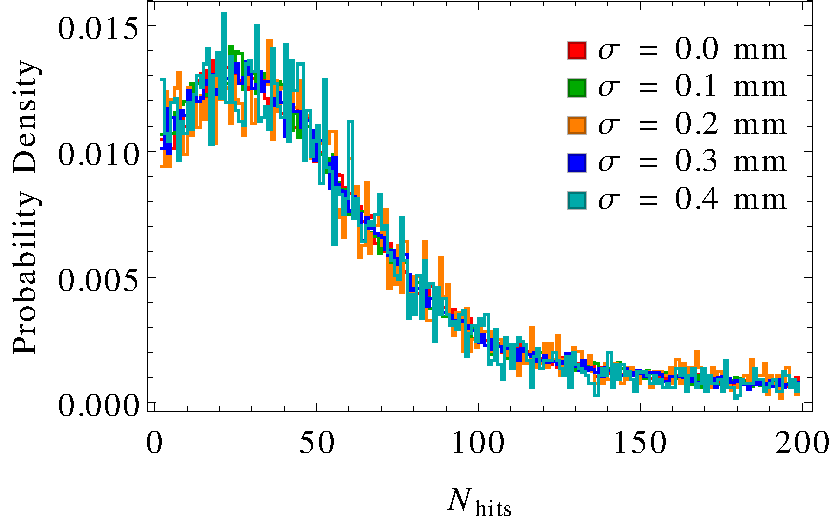
\includegraphics[width=\textwidth]{paint_uniformity_nhits_hists}
  \caption{Plot of NHit distributions for \Li beta decays inside a decay chamber with various paint surface roughnesses. The sigma value here is roughly the standard deviation of the fluctuations in thickness which were generated with a feature size of 1\,cm. The 0.2\,mm and 0.4\,mm plots have 10x fewer statistics due to simulation difficulties.}
  \label{fig:simulations}
\end{subfigure}
\hspace{0.5cm}
\begin{subfigure}{.38\textwidth}
  \centering
  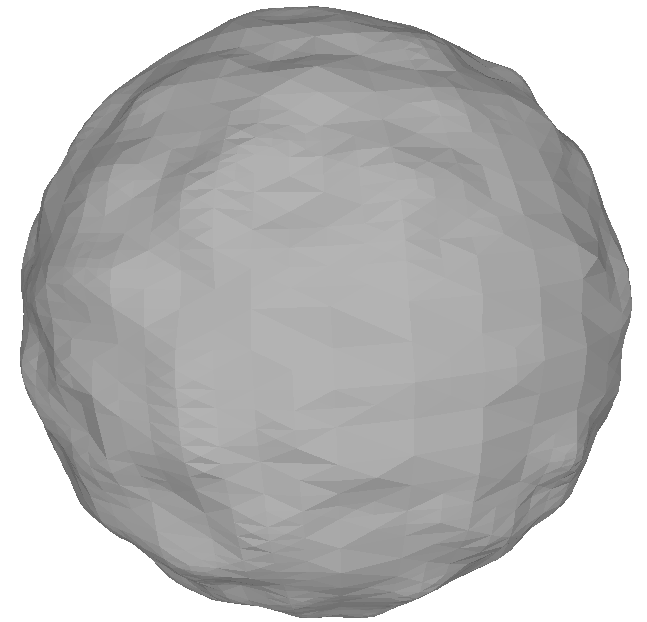
\includegraphics[width=0.85\textwidth]{0p5mm.png}
  \caption{Rendering of an STL defined paint surface imported into GEANT4 using perlin noise to simulate the expected roughness of the surface based on small scale tests. This is a sigma of 0.5\,mm which exaggerates the roughness enough to be clearly visible.}
  \label{fig:rough_sphere}
\end{subfigure}
\caption{Simulations with STL defined surfaces taking roughness and anisotropy in the paint layer into account show that neither has a strong effect on the NHit distributions.}
\label{fig:stltests}
\end{figure}

By generating stereolithography (STL) surface definitions, which break an arbitrary surface down into triangles, and importing these into GEANT4, it was possible to simulate how paint roughness or anisotropy would change the peak NHits. Figure~\ref{fig:stltests} summarizes the result that the expected roughness and anisotropy had no significant effect on the mean NHit. Since events are uniform in the decay chamber volume, and hence any individual beta sees a distribution of thicknesses of paint based on initial position and direction regardless of surface imperfections, the fact that these effects do not contribute strongly makes sense. Therefore it was only necessary to establish the mean paint thickness accurately to properly simulate the NHits distribution.

\begin{figure}[h!]
\begin{subfigure}{.45\textwidth}
  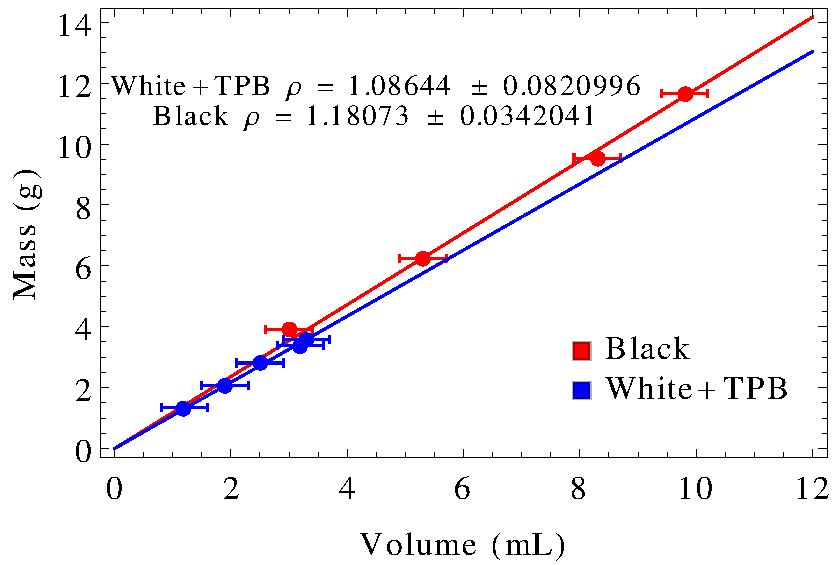
\includegraphics[width=\textwidth]{paint_density}
  \caption{Summary of density fit for black and white+TPB paint layers. The uncertainty on the mass of the samples was insignificant, and therefore the largest source of error was the volume measurement which was done with water displacement in a graduated cylinder with 0.2\,mL divisions and a tolerance of 0.2\,mL.}
  \label{fig:paintdensity}
\end{subfigure}
\hspace{0.5cm}
\begin{subfigure}{.45\textwidth}
  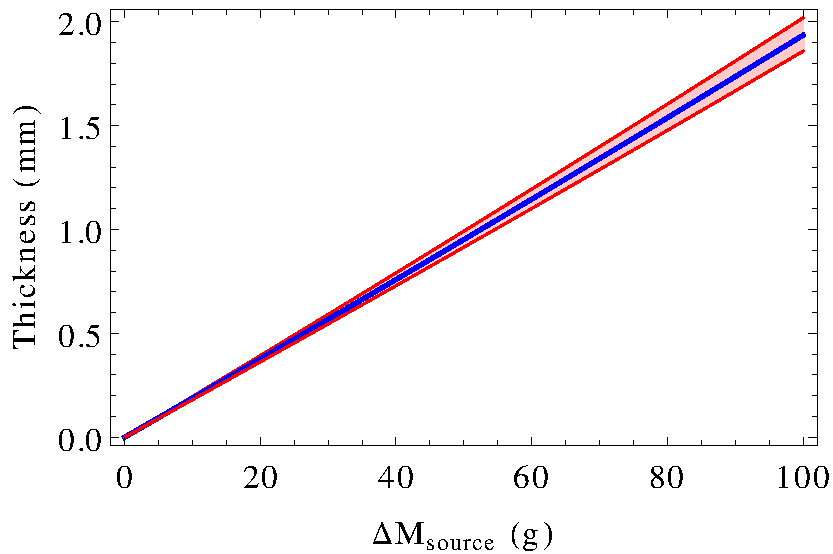
\includegraphics[width=\textwidth]{paint_rough_thickness}
  \caption{Assuming a simple uniform coverage model in the geometry of the source, this shows the mean and uncertainty on a thickness prediction for black paint given a measured change in the mass of the source. This can be further refined by taking into account non-uniform coverage. }
  \label{fig:paintthickness}
\end{subfigure}
\caption{Paint density data used in the weight to thickness conversion and a preliminary estimate of how well the calculation will work.}
\label{fig:weightmeasure}
\end{figure}

Many options for directly measuring the paint layer thickness were explored and ultimately rejected based on cost or lack of required precision. The final decision was to infer the paint thickness from the change in mass of the source before and after painting each layer. With a total source weight of 8.2\,kg and an expected total paint weight of 50\,g this required a scale capable of weighing 0.1\,g on top of 10\,kg so that uncertainty in weight was not a dominant source of error. The densities of the dry paint used in the black and white layers were fit using volume and mass measurements of small dry samples. These density results are summarized in Figure~\ref{fig:paintdensity}, and errors on these densities were the dominate sources of error for the thickness calculation. 

Figure~\ref{fig:paintthickness} gives a rough projection of estimated paint thickness for a given change in source mass. To do this conversion the change in mass must be converted to a paint volume, and the volume must be converted into a thickness using some model for how the paint coats the surface of the decay chamber. Using the source designs a model of paint coverage was developed as described in Figure~\ref{fig:surfacemodel} which ignores surface roughness since this should average out to the mean thickness. Based on small scale tests the expected anisotropy should lead to the neck area being roughly twice as thick as the thinnest section opposite the neck, however according to this model an uncertainty in anisotropy does not significantly change the inferred mean thickness. Ultimately this measurement procedure for the test source led to an inferred thickness of $1.02\pm0.04$\,mm, or approximately a 4\% uncertainty on the peak NHits.

\begin{figure}[h!]
\centering
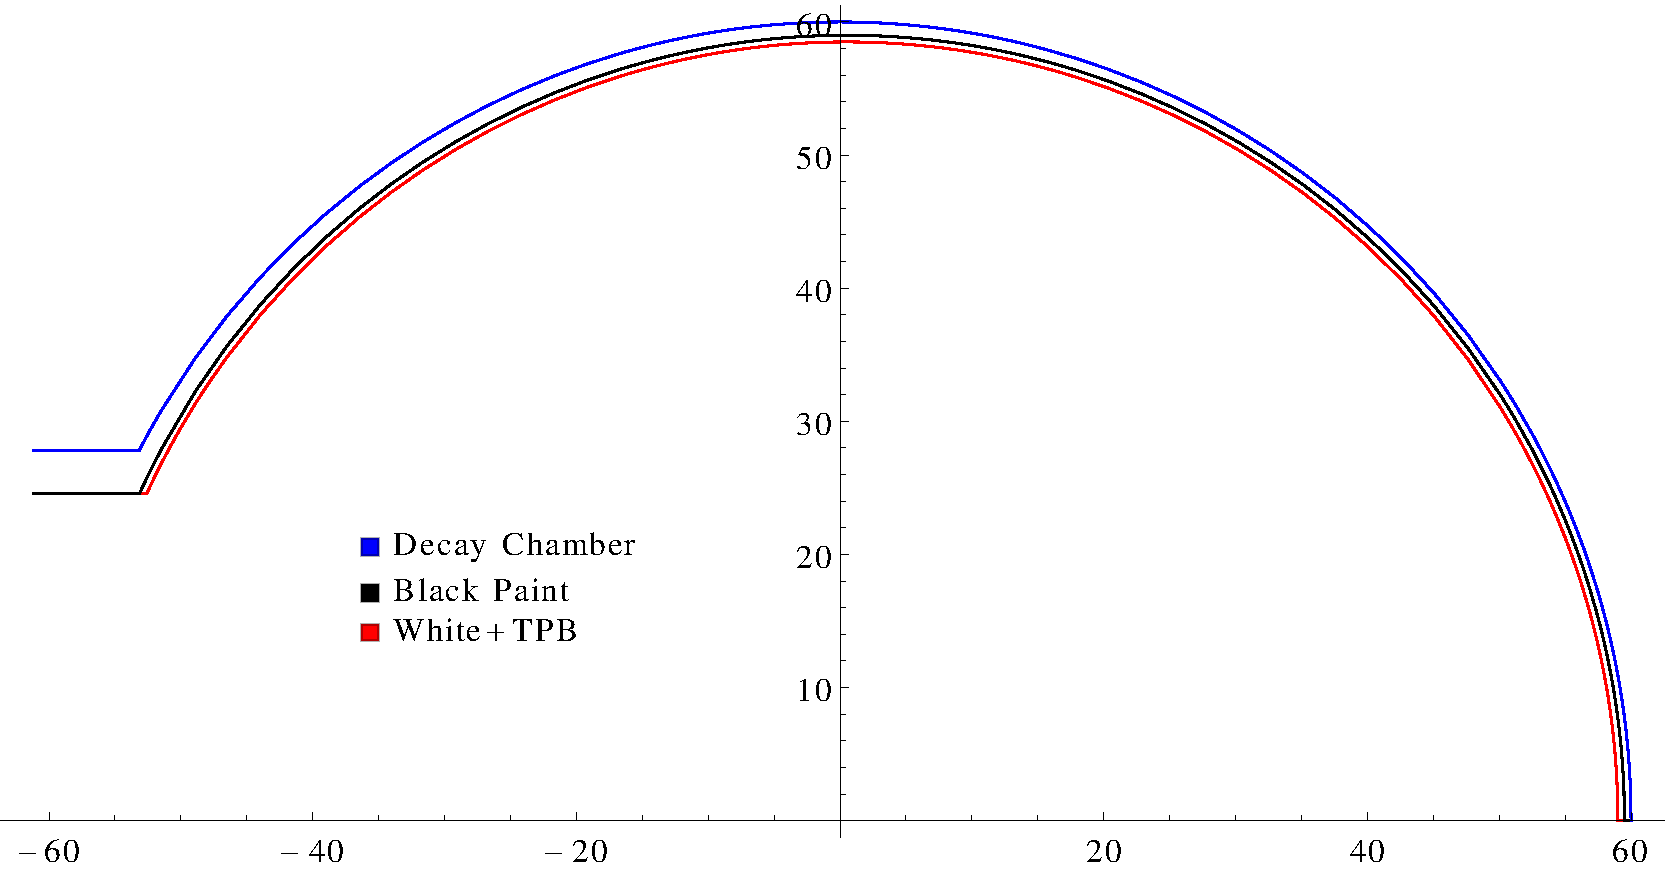
\includegraphics[width=0.7\textwidth]{paint_model}
\caption{The cylindrical profile of the full coverage model is shown here. This was revolved numerically to calculate the volume and hence the mass of the paint for a particular set of parameters to get a mass to thickness lookup table. Anisotropy in the paint thickness is accounted for by offsetting the inner surface of the black paint layer by some amount. In small scale tests this offset was empirically approximately half the mean thickness of the paint, and using this model it was verified that uncertainty in this anisotropy contributed a negligible uncertainty to the estimated mean thickness. The parameters for this profile are a black thickness of 1.0\,mm, anisotropy offset of 0.5\,mm, and white thickness of 0.5\,mm. }
\label{fig:surfacemodel}
\end{figure}

\subsection{PMT assembly potting}
The PMT used for the source is the Hamamatsu H11432-100 which has an integrated high voltage supply that requires only low voltage (+5V) to operate. This is advantageous because there will be helium gas inside the source which would form a plasma if exposed to high voltage, and this configuration does not require providing high voltage via the umbilical. However, the PMT supply itself does not come potted and helium gas could leak inside resulting in a plasma that would damage the PMT and possibly the source. To prevent this the high voltage supply module was potted into an anodized aluminum potting sleeve with Sylgard~184, a silicone encapsulate, which was also allowed to fill the cavity containing the supply and around the body of the PMT as shown in Figure~\ref{fig:potting}. To ensure the encapsulate fully filled the cavities the assembly was placed in a soft vacuum between applications of encapsulate to assist in removing air that may have been trapped. This entire potted PMT assembly fits directly into the neck sleeve and contains the o-rings that isolate the decay chamber from the rest of the source, so this potting serves the additional purpose of making the PMT assembly into a solid part to isolate the decay chamber from the rest of the source. 

\begin{figure}
\begin{subfigure}{.385\textwidth}
  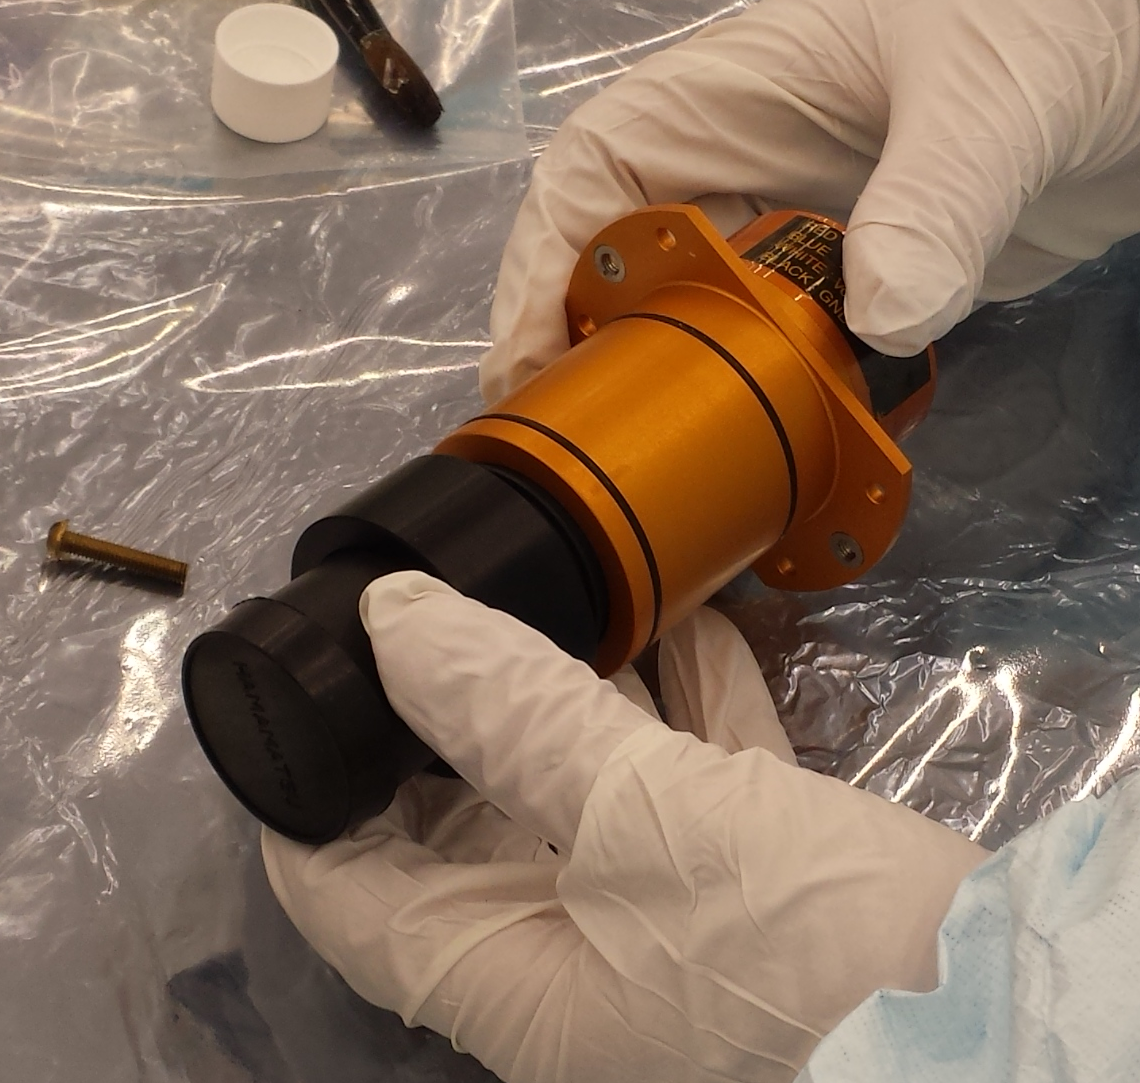
\includegraphics[width=\textwidth]{potting_1.png}
  \caption{The PMT to be potted inside the anodized aluminum spacer (black) and anodized aluminum potting sleeve (orange).}
  \label{fig:potting_a}
\end{subfigure}
\begin{subfigure}{.305\textwidth}
  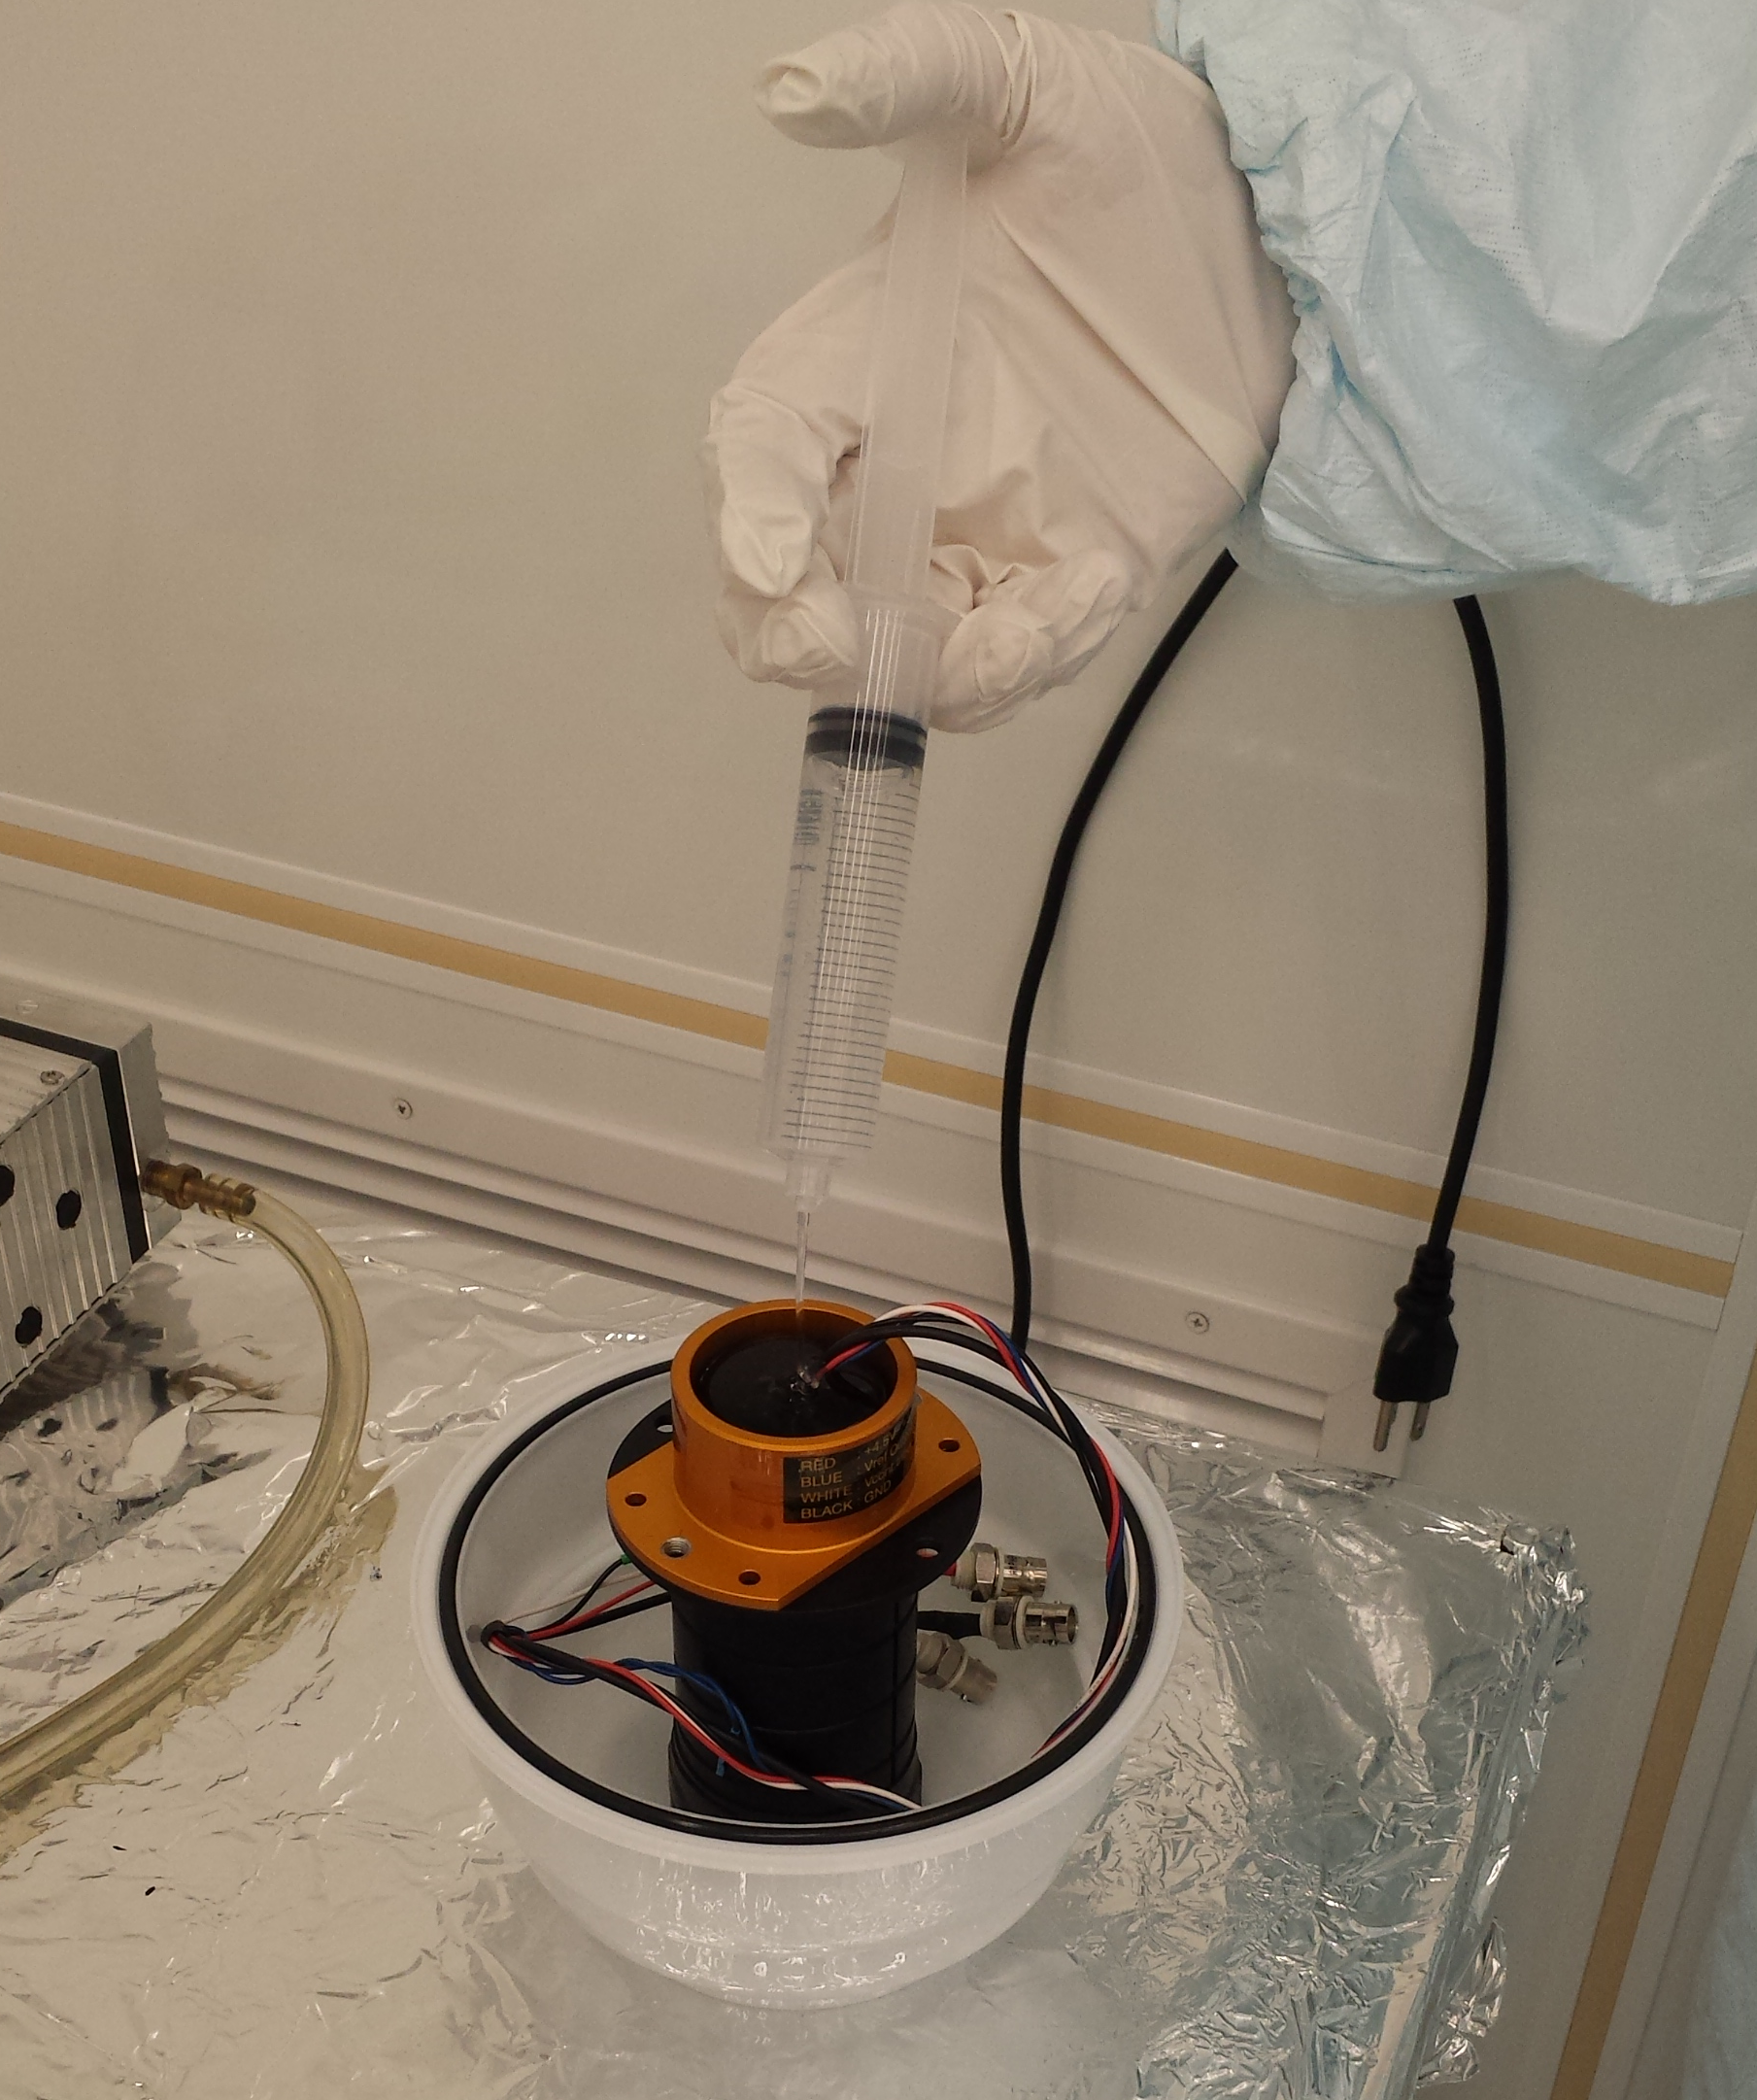
\includegraphics[width=\textwidth]{potting_2.png}
  \caption{Encapsulate added in stages with vacuum between to fill areas with trapped air}
  \label{fig:potting_b}
\end{subfigure}
\begin{subfigure}{.29\textwidth}
  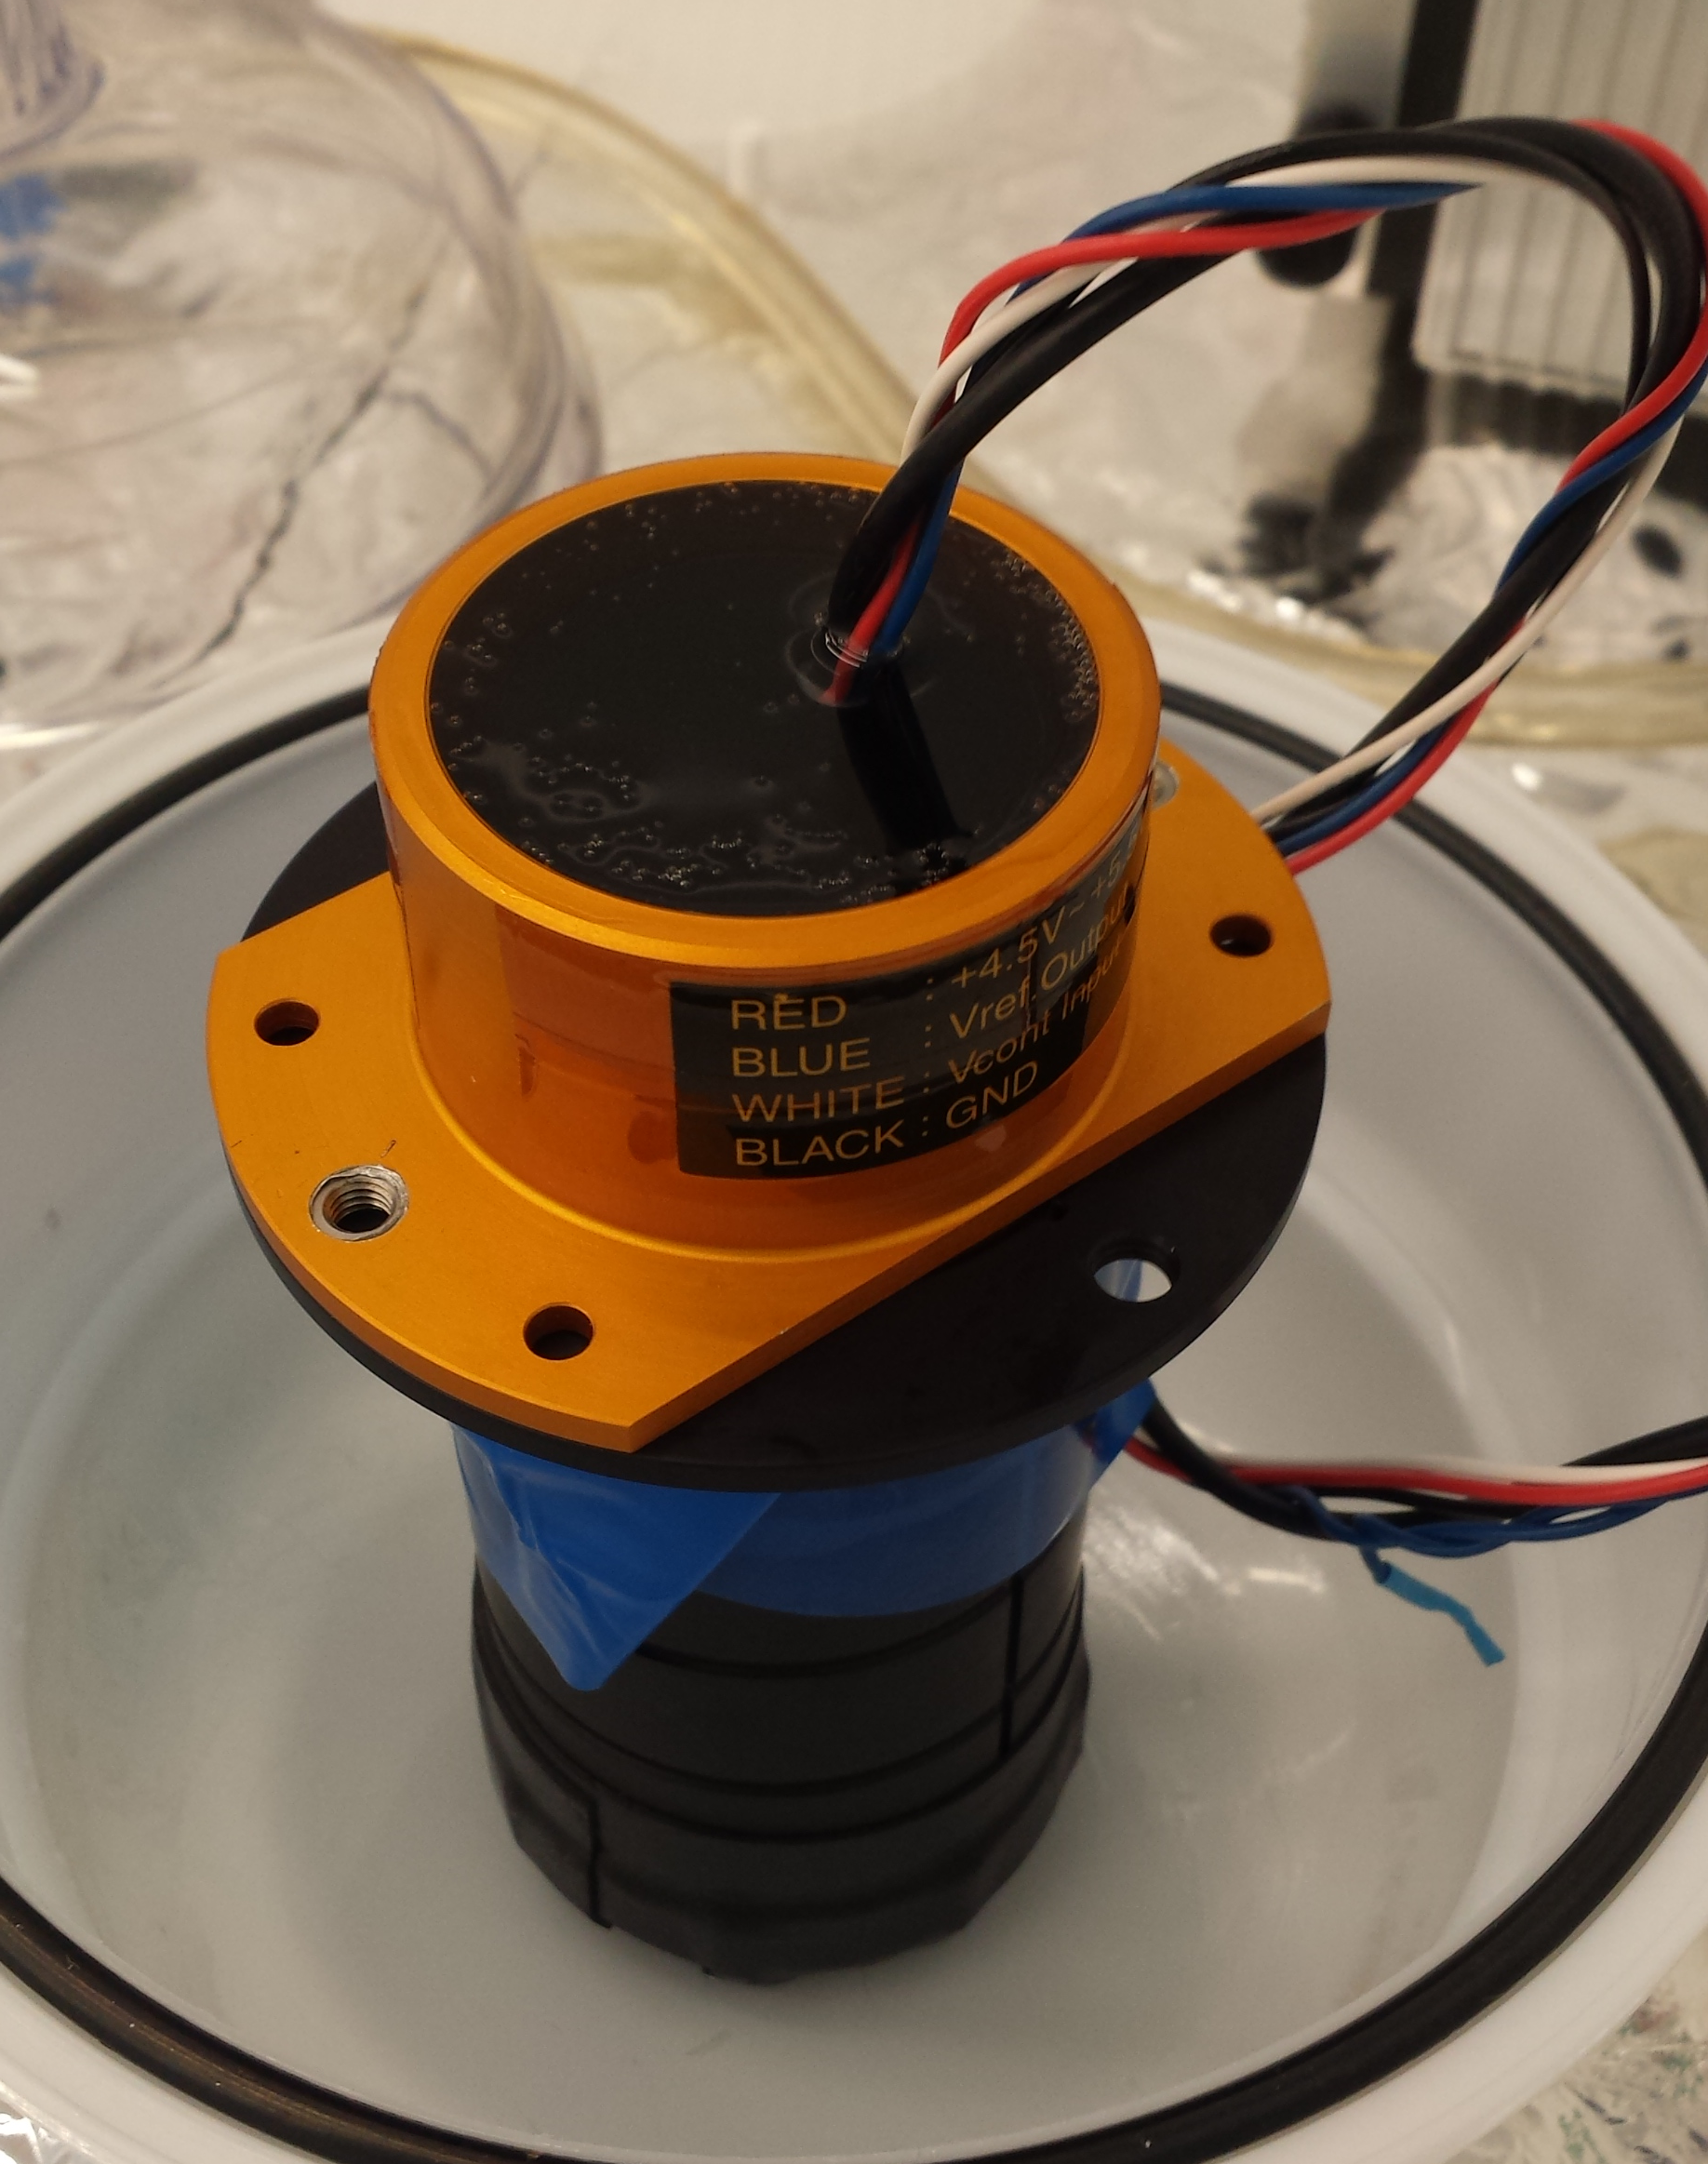
\includegraphics[width=\textwidth]{potting_3.png}
  \caption{Finally the encapsulate was allowed to cure in the clean room.}
  \label{fig:potting_c}
\end{subfigure}
\caption{Potting of the PMT into the anodized aluminum components for the final source. All work was done in the class-1000 clean room at LBNL.}
\label{fig:potting}
\end{figure}

\section{Tests and radon emanation estimation}
\label{chap:tests}

This section describes the tests that were done on the source and the source materials. We also perform a first estimate of the radon emanation of the completed source. Table~\ref{tab:testoverview} gives an overview of the tests and calculations, with the current status and conclusion. See the following subsections for all details on the test procedures and results. 

\begin{table}[p]
\centering
%\small
\normalsize
\begin{tabular}{|p{2.7cm}|p{6cm}|p{7.3cm}|} \hline
Test/estimate           & Outcome  & Conclusion \\ \hline

Emanation calculation, see~\ref{sec:emanation}   
                        & A first estimate of the total radon emanation yields $<92.5$ atoms/day.
                        & The total radon budget for the SNO+ sources is yet to be determined. We feel that the Cherenkov source emanation upper limit is low enough to fit inside such a budget. The steel will be polished and the acrylic sphere has been stored in a N-flushed radon-resistant bag.\\ \hline   

Material counting, see~\ref{sec:matcounting}      
                        & We found high $^{40}$K levels in both the TiO white paint ($\sim$111\,ppb) and the Sylgard silicon ($\sim$6.7\,ppb). 
                        & \multirow{2}{7cm}{The high $^{40}$K levels in the lining and the silicon and their incompatibility with the LS adds an additional risk to the detector should the source break while in the detector. We feel that the source is sufficiently sealed and strong to allow for a safe deployment. See also Section~\ref{sec:integrity}.} \\ \cline{1-2}
                        
Material compatibility, see~\ref{sec:comptest}  
                        & We found the decay chamber lining materials and the Sylgard silicon to be incompatible with LAB. The silicon shows swelling and all materials show a change in absorption. 
                        & \\ \hline
                                             
Threaded insert torque, see~\ref{sec:inserts}
                        & No change in stress-patterns (loss of torque) was observed after several months for a screw and screw-insert combination torqued to 14\,ft/lbs.
                        & The torque applied to the Cherenkov-source screws will be 7\,ft/lbs. The reference piece will be regularly checked for any loss in torque. We feel that these screws+threaded screw-inserts are strong enough to confidently attach the steel housing to the acrylic decay chamber. \\  \hline
                        
Decay chamber lining, see~\ref{sec:liningtest}
                        & The light leak from scintillation photons is estimated to be fewer than 1 photon in 50 events.
                        & This light-leak will have no impact on the Cherenkov source estimate of the light collection efficiency. \\ \hline

Decay chamber He leak, see~\ref{sec:heleak}
                        & During the He-leak testing, a leak rate of 6.2$\times10^{-9}$\,torr l/s. was seen after about 2 minutes. No change in rate is observed when spraying Helium along the bond-plane. & We conclude that there is no leak in the decay chamber, this includes the place where the flange o-ring passed over the bond-plane twice. \\ \hline

Tag PMT test, see~\ref{sec:tagpmt} 
                        & The potting of the PMT reduced the PMT gain. Triggering will most likely need to happen above 5\,PE. 
                        & A large number of primary scintillation photons ($\sim$20K) is expected but only wavelength-shifted photons will be detectable. The wavelength shifting efficiency and reflectivity of the decay chamber lining is not known. An on-site dark-box test is planned to measure the PMT tagging efficiency. \\ \hline
\end{tabular}
\caption{\label{tab:testoverview} Overview of the Cherenkov source testing.}
\end{table}

\subsection{Radon emanation and Backgrounds}
\label{sec:emanation}
A first pass radon emanation estimate can be calculated by considering the surface area of stainless steel and acrylic that will be exposed to the cover gas and target material. Estimates for the radon emanation of the UI used a measurement of $4.60$ $\mu$Bq m$^{-2}$ for stainless steel \cite{kormos:2015}. The SNO stainless steel limit was $< 5$ mBq m$^{-2}$ and for acrylic $< 1.6$ mBq m$^{-2}$ \cite{Liu:1993}. The source, assuming a full size stainless steel housing, has an exposed stainless steel surface area of $0.15$ m$^2$, and exposed acrylic surface area of 0.20 m$^2$. Assuming the stainless steel housing remains at its full size and can reach the cleanliness standards assumed in the UI emanation estimate, this leads to a total radon emanation from the exposed surfaces of the source to $<28$ atoms/day where this limit is grossly dominated by the limit on the acrylic radon emanation. The radon emanation rate for stainless steel is significantly lower in the source used by the UI document than number used by SNO, which either means the UI estimation is unrealistic or the SNO limit was very conservative. Using the limits from the SNO measurements we would expect $<92.5$ atoms/day.

Since the source construction did not involve any explicit sources of radioactivity and was done in a clean room environment, the surface of the source is expected to be free of any gross radioactive contamination. Further, the acrylic sphere has been stored in nitrogen flushed radon proof bags to limit the plating of radon daughters onto these surfaces, so leaching into the target material is not expected to be a large effect.

\subsection{Material counting}
\label{sec:matcounting}
See Table \ref{tab:counting} for counting results for materials used in the source. The nuclear activation analysis (NAA) results were exposed at the McClellan Nuclear Research Center and counted at UC Davis. The low background counting facility at LBNL directly counted the UVA acrylic.
\begin{table}[h!]
\centering
\begin{tabular}{|l|l|l|l|l|l|} \hline
                    Material       & Mass in source & Method    & $^{238}$U     & $^{232}$Th    & $^{40}$K      \\ \hline
 \multirow{2}{*}{}  UVA acrylic    & 8096.7\,g & NAA    & $<$81\,ppb    & $<$24\,ppb   & $<$2.1\,ppb   \\ \cline{3-6}
                                   & & Direct & $<$0.8\,ppb (early)&$<$0.8\,ppb (early)& $<$0.4\,ppm \\ \hline
                    Black paint    & $\approx 50$\,g & NAA    & $<$252\,ppb   & $<$37\,ppb   & $<$3.9\,ppb           \\ \hline
                    TiO paint      & $\approx 1.5$\,g & NAA    & $<$2.8\,ppm   & $<$189\,ppb  & $111.5 \pm 8.6$\,ppb           \\ \hline
                    TPB            & $\approx 4$\,g & NAA    & $<$0.8\,ppm   & $<$237\,ppb   & $<$47.1\,ppb  \\ \hline
                    Sylgard silicon& $\approx 200$\,g & NAA    & $<$116\,ppb   & $<$48\,ppb   &6.7$\pm$1.5\,ppb\\ \hline
\end{tabular}
\caption{\label{tab:counting} Cherenkov source material counting results. Approximate masses are estimates from the test source that should be approximately the same for the final source upon its completion.}
\end{table}

From all the materials, only the potassium levels for the TiO white paint and the Sylgard silicon have been measured. All the other measurements yielded upper limits. Except for the UVA acrylic, none of the tested materials are expected to come into contact with the UPW or LS inside the AV. We feel that the source is sufficiently sealed and strong to allow for safe deployments inside the detector. There was no gross contamination found in the UVA acrylic.

\subsection{Material compatibility tests}
\label{sec:comptest}
Three samples were tested for compatibility with LAB-PPO by the technical support team at SNOLAB: the potting material (Sylgard~184), a UVA acrylic sample with black paint and one with both black and white paint. The white paint has TPB mixed in. The materials were soaked in a few 100\,mL of 2g/L PPO-LAB for 1 month. A control sample consisting of the default 2g/L PPO-LAB was scanned with the samples and used as a comparison. Deviation from the control is observed in all of the samples indicating incompatibility. None of the materials tested will be in contact with the UPW or LAB in normal operation mode.
\begin{enumerate}
    \item Sylgard~184, tested for deformation, specifically swelling and LAB-PPO absorbance changes.
    \begin{itemize}
        \setlength{\itemsep}{-0.2cm}
        \item After 1 day: slight increase in absorbance but samples increased in size and weight.
        \item After 1 week: a further deviation in absorbance and increase in size and weight.
        \item After 1 month: continuation of the swelling and absorption deviation. 
    \end{itemize}
    \item UVA acrylic + black paint, tested for LAB-PPO absorbance changes.
    \begin{itemize}
        \setlength{\itemsep}{-0.2cm}
        \item After 1 day: slight change in absorbance.
        \item After 1 week: a slightly higher absorbance.
        \item After 1 month: continued to deviate from the control.
    \end{itemize}
    \item UVA acrylic = black paint + TiO paint + TPB, tested for LAB-PPO absorbance changes.
    \begin{itemize}
        \setlength{\itemsep}{-0.2cm}
        \item After 1 day: a shift in wavelength is visible.
        \item After 1 week: additional deviation and shift in wavelength.
        \item After 1 month: continued to shift. A new peak was also observed in the $\sim$658\,nm region.
    \end{itemize}
\end{enumerate}
For the full technical report of the compatibility test, see~\cite{lina:2015}.

\subsection{Threaded inserts}
\label{sec:inserts}
The decay chamber is attached to the source steel housing by means of 8 screws (1/4-20 socket head cap screws), see Figure~\ref{fig:drying}b and also \cite{wallig:2015}, page 14. It was decided to use threaded inserts to eliminate the outward force created by directly threading the acrylic. These inserts are glued in place with Weld-On\,\#40. A test-piece was made in which two screws were torqued to 14\,ft/lbs, one using a thread insert and the other using direct threading (plain tapped hole). The piece was then observed through polarized light. The plain tapped hole showed the stress radiating out from the threads as well as irregular stress patterns angular to the mating surface. The glued-in insert showed more even stress patterns angular to the mating surface. After a while, the plain tapped hole lost some torque. Figure~\ref{fig:nutts} shows the test-piece (months after the screws were put in place) as viewed through polarized light. The torque applied to the Cherenkov-source screws will be 7\,ft/lbs.

\begin{figure}
\center{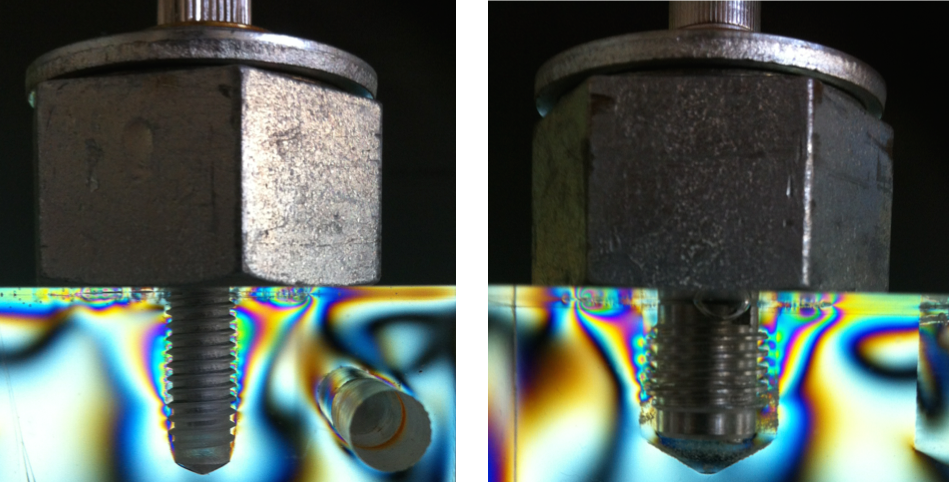
\includegraphics[width=.6\textwidth]
{Screw-inserts.png}}
\caption{\label{fig:nutts} Testing glued (right) versus drilled (left) screw grooves, as viewed through polarized light. The drilled grooves have lost some torque while the insert is still tight and showing the torque on the plastic. }
\end{figure}

\subsection{Decay chamber lining tests}
\label{sec:liningtest}
The light tightness of the decay chamber lining was validated on the full scale test source. To do this, the test source was placed in a dark-box with the center of the source 12" away from a 10" Hamamatsu R7081 HQE PMT which has the SPE peak clearly separated from the noise. 
\begin{figure}
        \begin{subfigure}{0.49\textwidth}
                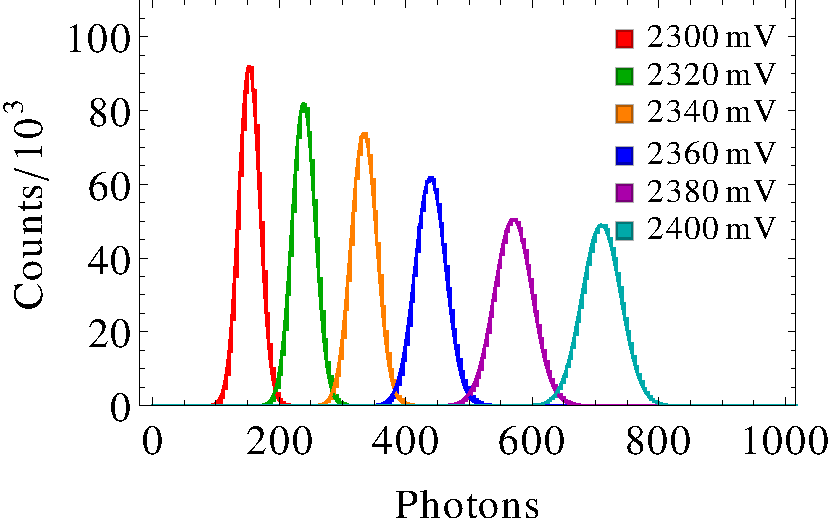
\includegraphics[width=\textwidth]{led_calibration_raw}
                \caption{Raw detected photon data at various voltages.}
                \label{fig:ledRAW}
        \end{subfigure}%
        \hspace{0.2cm}
        \begin{subfigure}{0.49\textwidth}
                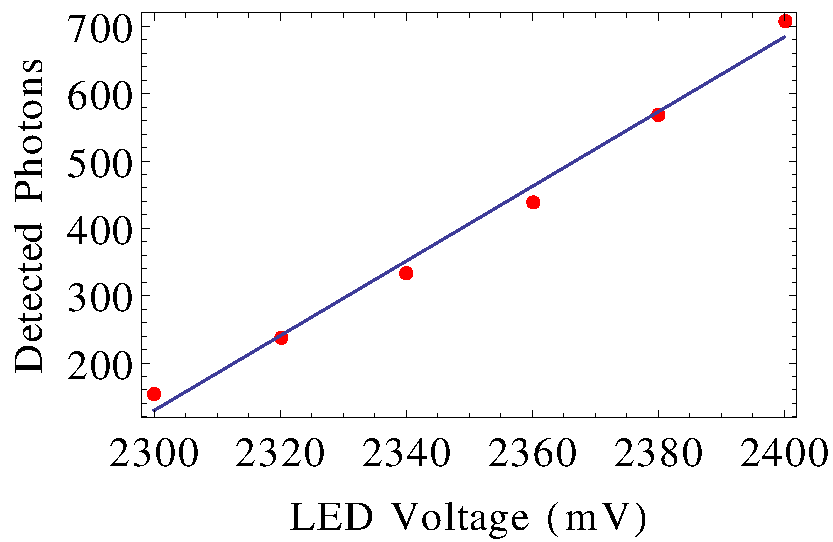
\includegraphics[width=\textwidth]{led_calibration_fit}
                \caption{Fit to the peaks of the photon distributions plotted against pulse voltage.}
                \label{fig:ledFit}
        \end{subfigure}
        \caption{Calibration data for the LED used to test the light tightness of the decay chamber lining. LED intensity was measured at 50\,cm from a R7081 10" PMT. The LED was pulsed at 50\,ns at various voltages.}
\label{fig:calibratedled1}
\end{figure}

A calibrated LED (see Figure \ref{fig:calibratedled1}) around the emission wavelength of TPB was placed in the center of the source with the neck blocked by an opaque rubber plug. This LED was pulsed on for 50\,ns intervals at various voltages one million times per LED voltage setting. The signal from the PMT was digitized and integrated with a per event pedestal correction to obtain a signal charge distribution. To cancel out systematics, the same process was repeated with the LED off to obtain a background charge distribution. The leaked light charge distribution was obtained by subtracting the background charge distribution from the signal charge distribution. There were no samples in the background subtracted charge distribution that appeared to correspond to multi-photon events, so each event that registered charge in the leaked light charge distribution was counted as a single leaked photon. The sum of leaked photons for the million events at each voltage are shown in Figure \ref{fig:lightleak}. 
\begin{figure}
        \begin{subfigure}{0.47\textwidth}
                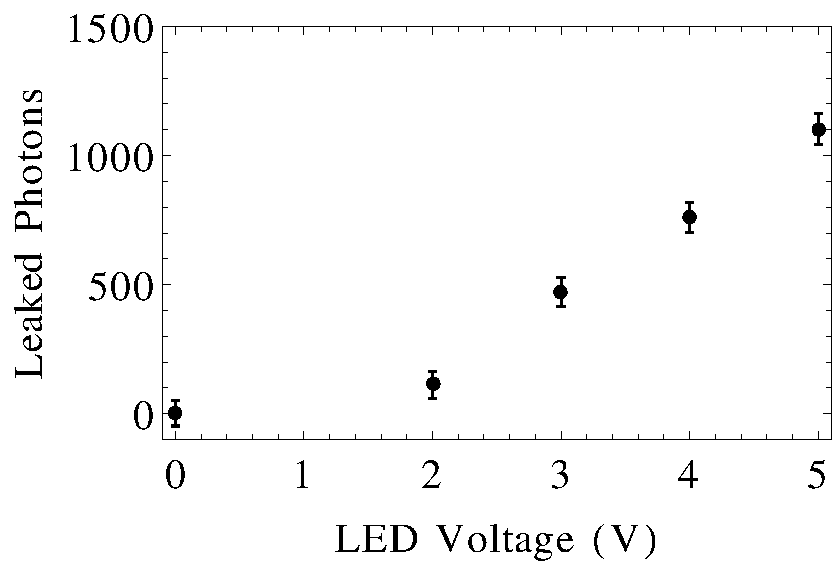
\includegraphics[width=\textwidth]{leakedphotons}
                \caption{Raw data showing the total number of photons detected by the PMT at the different led voltages tested where each datapoint is the sum of 1,000,000 events. Note the expected linear trend after the LED turns on around 2V. The uncertainties here are statistical measurement error.}
                \label{fig:lightleak}
        \end{subfigure}%
         \hspace{0.2cm}
        \begin{subfigure}{0.49\textwidth}
                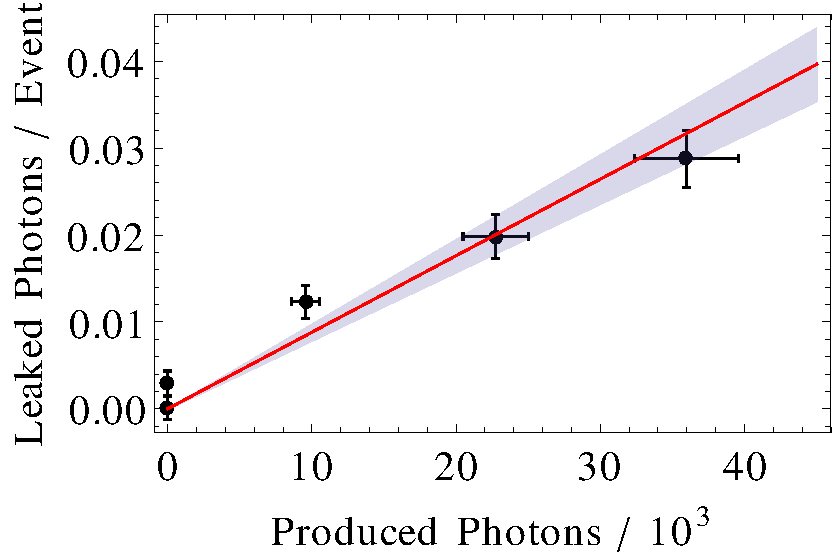
\includegraphics[width=\textwidth]{light_leak}
                \caption{Data showing the expected number of photons to leak per event from the source given some number of thousands of photons produced per event in the source.}
                \label{fig:eventleak}
        \end{subfigure}
        \caption{Summary of the data collected on the light tightness of the decay chamber lining. The actual expected light leak is, conservatively, on the order of 1 photons in 50 events.}
\label{fig:calibratedled2}
\end{figure}

To determine the total light leak of the source assume that the light leaking from the source is isotropic such that the PMT sees only a fraction of the total $4\pi$ light leak. Since the LED inside the source was pointed directly at the PMT, this is a conservative assumption. This along with dividing by the total number of events converts the y-axis of Figure \ref{fig:lightleak} to the y-axis of Figure \ref{fig:eventleak}. The calibration data in Figure \ref{fig:calibratedled1} shows the number of photons detected by the PMT without the source blocking the light from the LED. Correcting for the solid angle effect arising from the larger spot size of the LED compared to the solid angle of the PMT at 50\,cm gives the total number of photons produced by the LED when pulsed at 50\,ns at a particular voltage. This converts the x-axis of Figure \ref{fig:lightleak} to the x-axis of Figure \ref{fig:eventleak}. Therefore, Figure \ref{fig:eventleak} shows an upper limit for the expected leak per event with some average number of scintillation photons produced inside the decay chamber. This is an over estimate assuming perfect TPB efficiency, since any primary scintillation photons would be absorbed by the acrylic, but nonetheless puts an acceptable upper limit on the light leak to fewer than 1 photon in 50 events at our expected mean number of scintillation photons.

\subsection{He leak test of decay chamber}
\label{sec:heleak}
The decay chamber for the final source was tested for leaks using ultra-pure Helium as tracer-gas. The Helium-leak checker used was INFICON UL1000, which was calibrated after a one-hour warm-up time. The baseline achieved was 1.4$\times10^{-11}$\,Torr\,l/s. After mounting the Cherenkov decay chamber on the flange, see Figure~\ref{fig:HeLeakCheckSetup}, a leak rate of 6.2$\times10^{-9}$\,Torr\,l/s. was seen after about 2 minutes. No increase in leak rate was observed when spraying Helium over the source and close to the flange. In a second stage, a clear bag was placed over the source. It was held shut at the bottom using clean-room tape. Then, the helium was injected into the bag. No increase in leak was observed over the course of 2 minutes. After 5 minutes, an increase of the leak rate was noticed, which is expected from permeation through the Viton o-ring inside the flange-attachment. We conclude that there is no leak in the decay chamber bond. This includes the location where the flange o-ring crosses the bond-plane twice.

\begin{figure}
        \centering
        \begin{subfigure}[b]{0.48\textwidth}
                \centering
                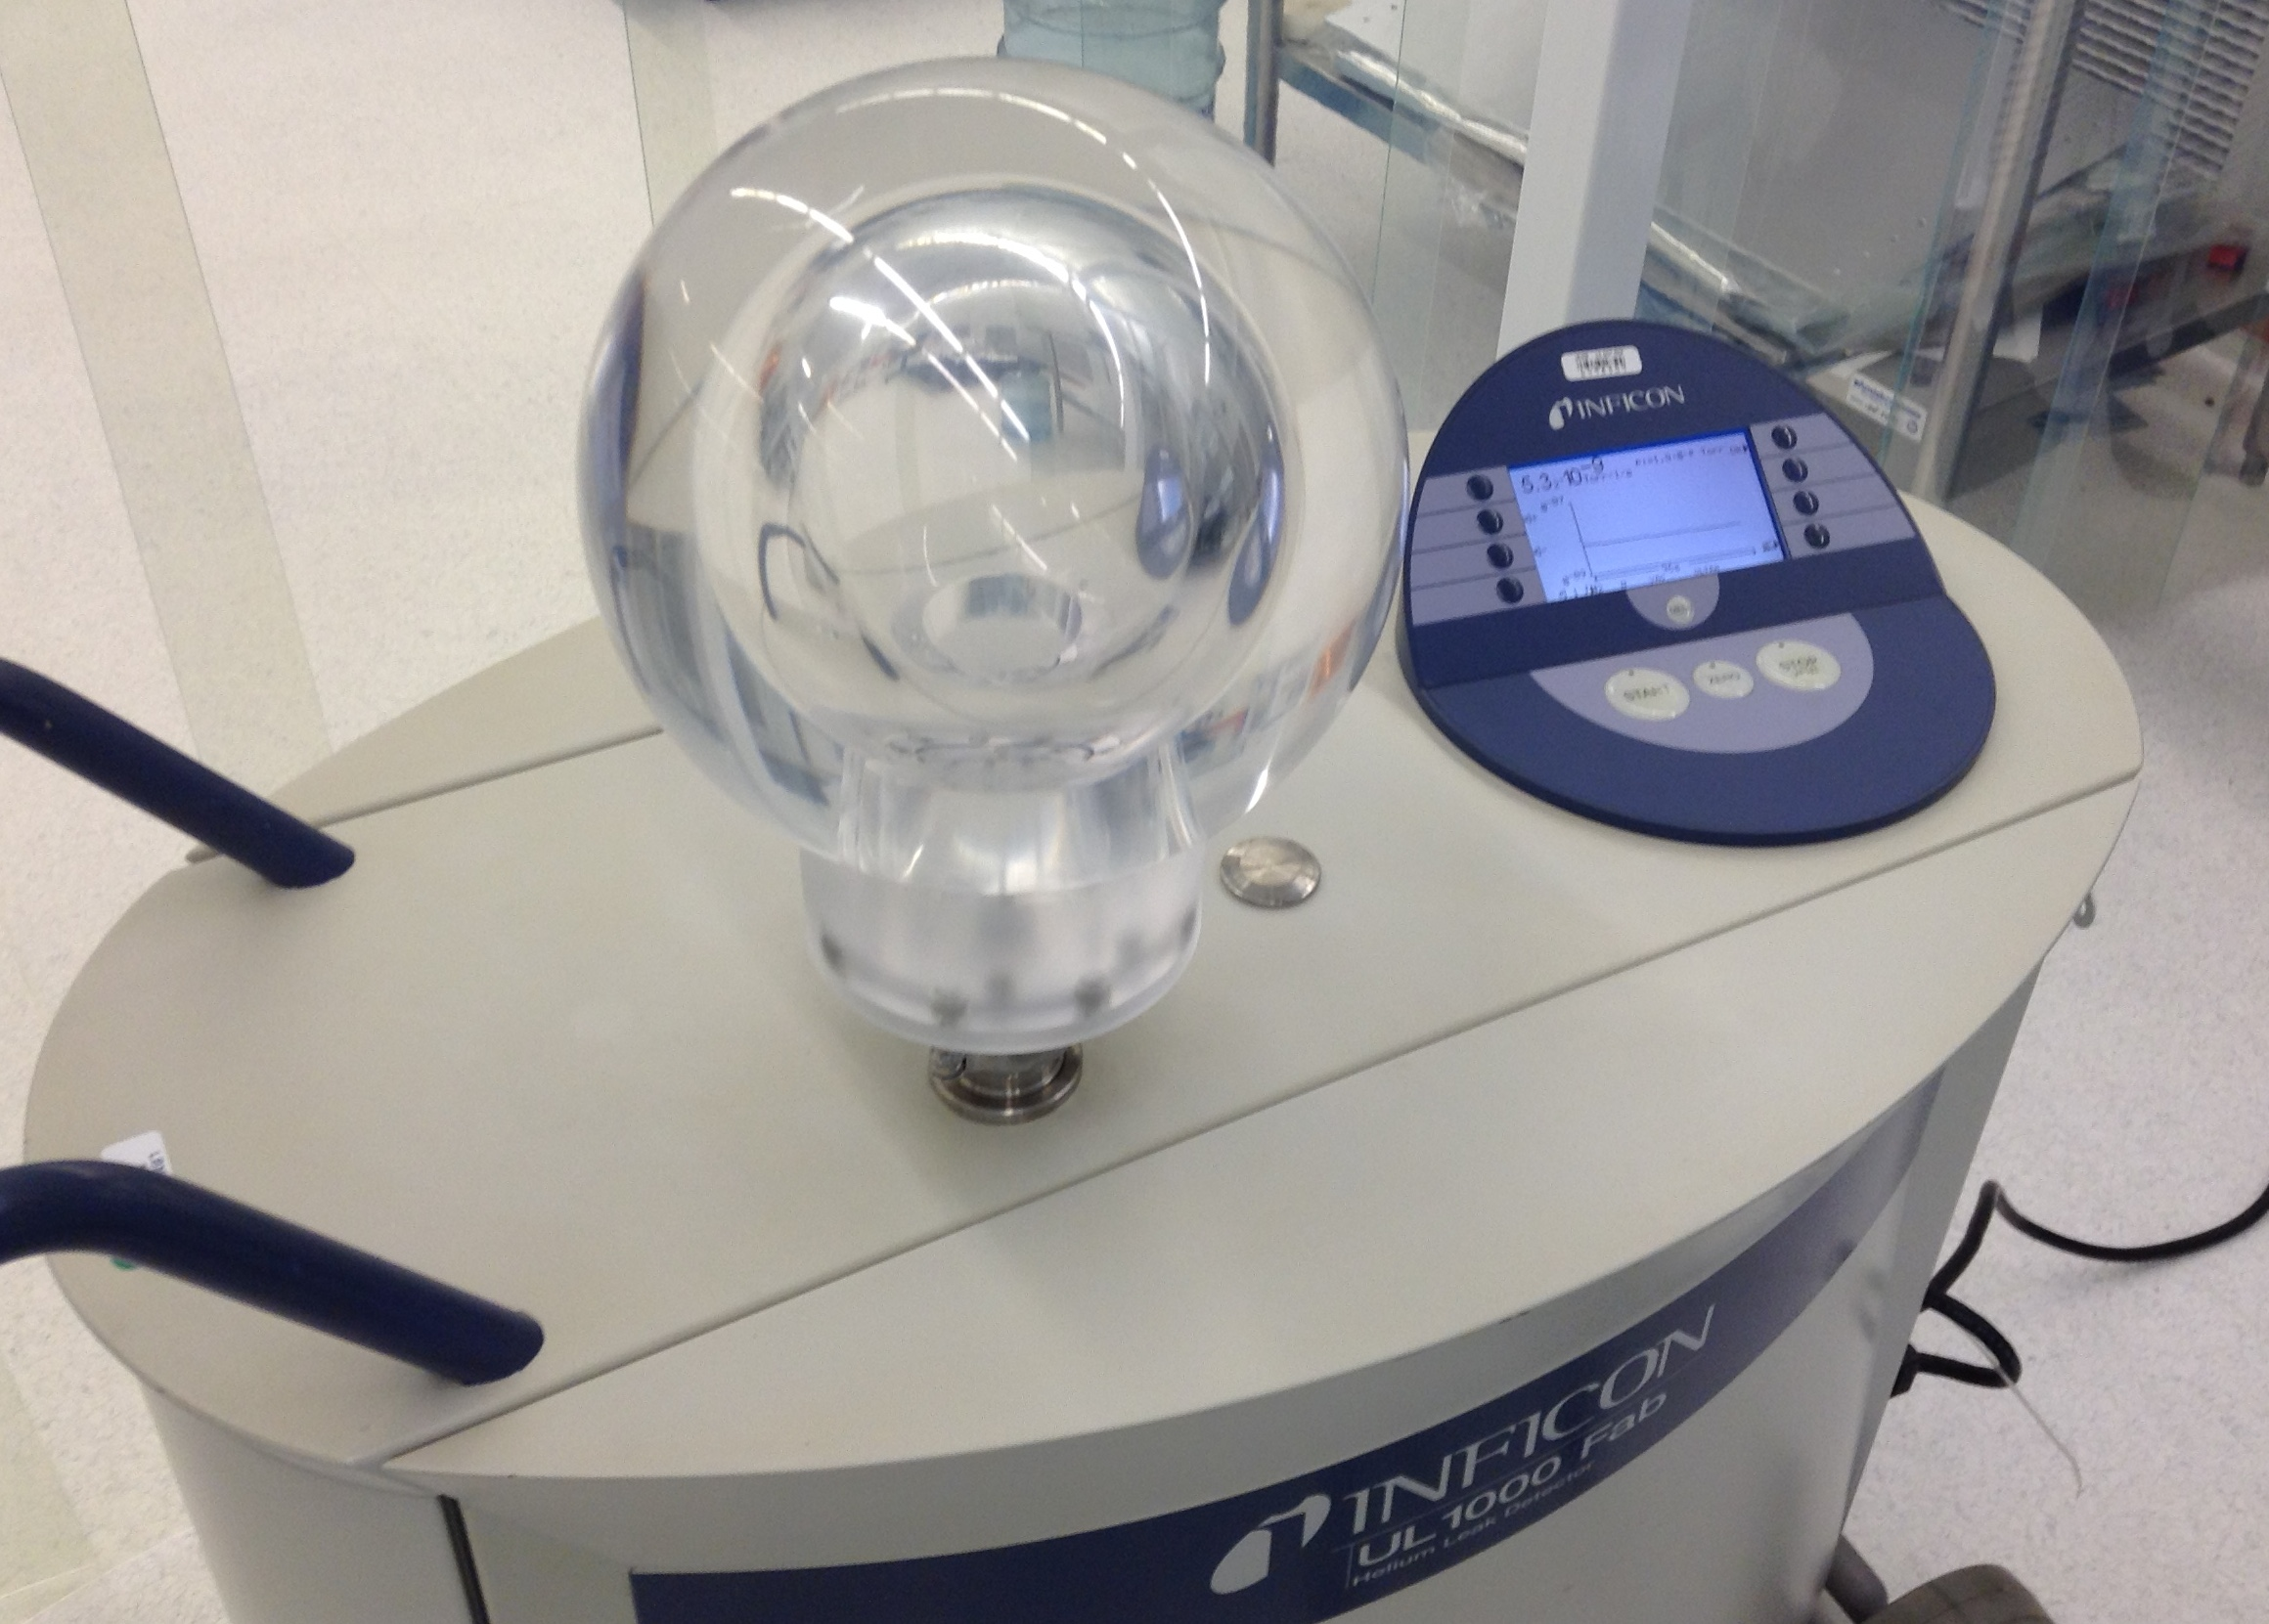
\includegraphics[width=\textwidth]{img_0328.jpg}
                \caption{}
                \label{fig:HeLeakCheckSetup}
        \end{subfigure}%
        \vspace{0.2cm}
        \begin{subfigure}[b]{0.45\textwidth}
                \centering
                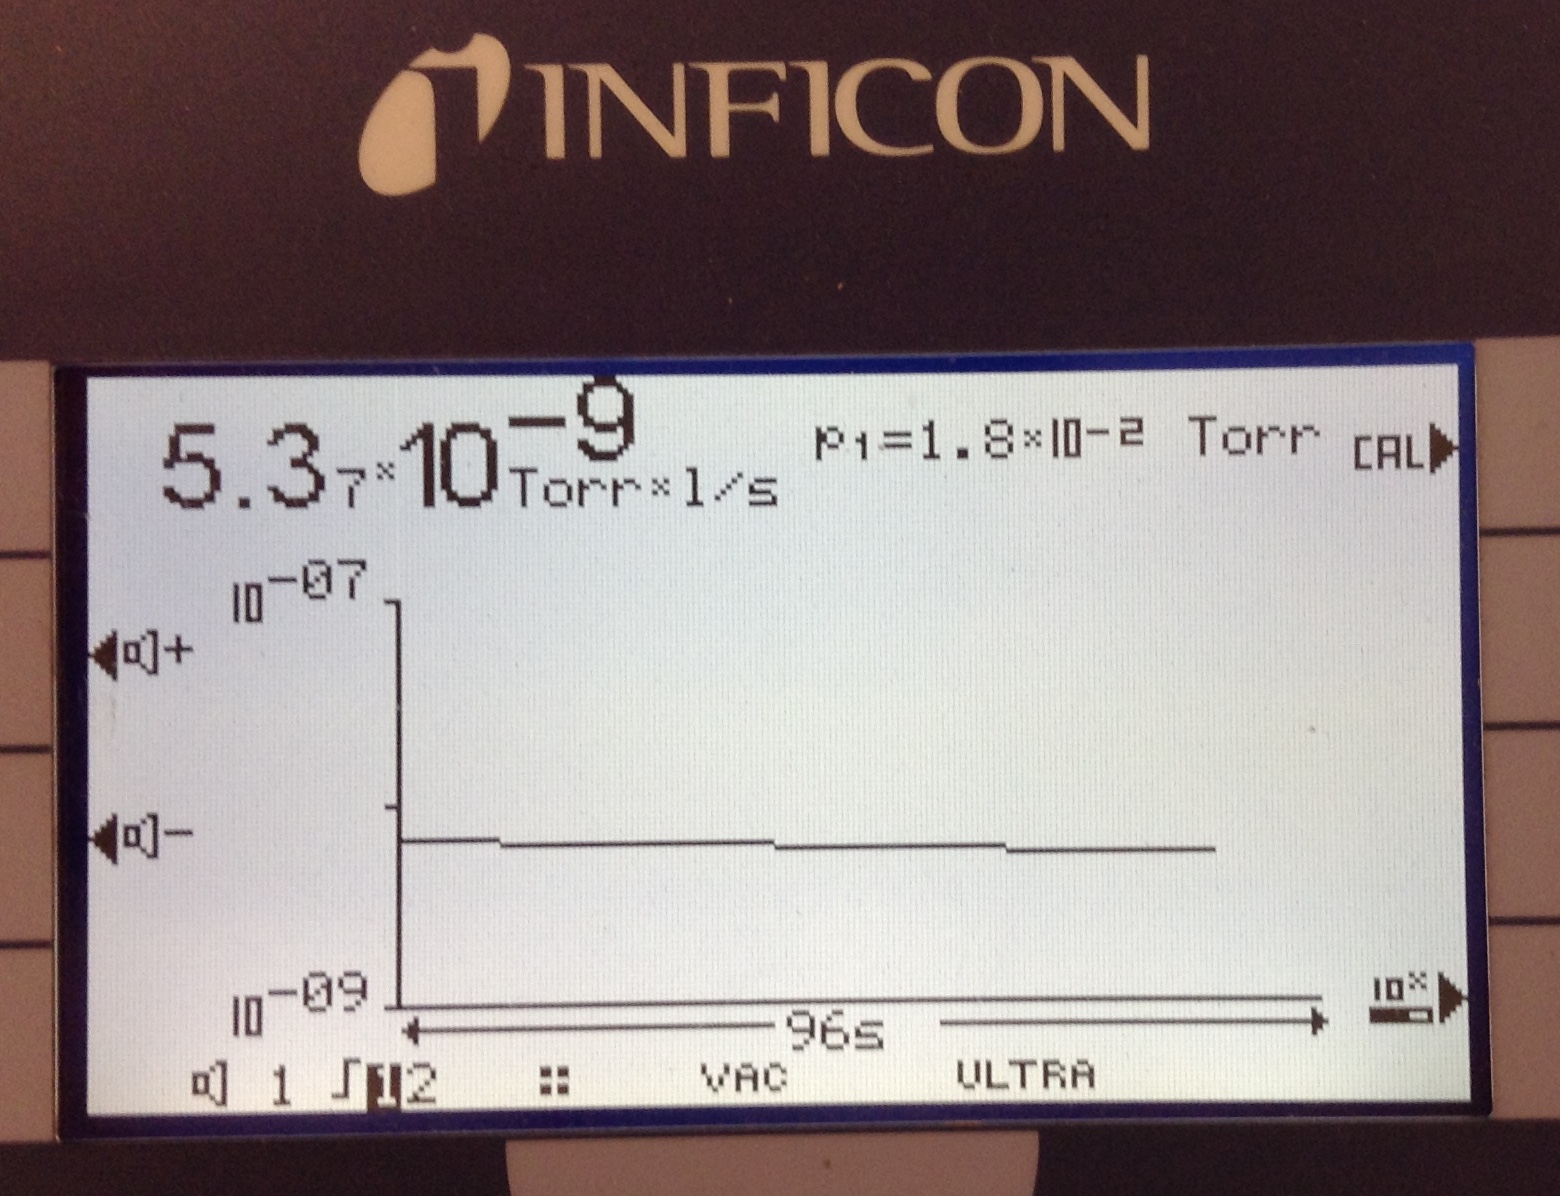
\includegraphics[width=\textwidth]{img_0326.jpg}
                \caption{}
                \label{fig:HeLeakCheckResult}
        \end{subfigure}
        \caption{Helium-leak checking of the decay chamber using INFICON UL1000 in the LBNL clean room.}
\label{fig:HeLeakCheck}
\end{figure}

\subsection{Tag PMT test}
\label{sec:tagpmt}
The H11432-100 PMT efficiency and gain were measured before and after potting into the PMT assembly both to ensure the PMT had appropriate sensitivity across a wide range of photon fluxes and to see what effect the potting had on the PMT. This was done by placing the PMT in a dark-box 50\,cm away from a calibrated LED. The LED was pulsed for 50\,ns at various voltages to change the photon flux. Figure~\ref{fig:pmttest} shows that the PMT is indeed sensitive over a large range of photon fluxes, however comparing Figure~\ref{fig:pmttest} to Figure~\ref{fig:pmtafterpotting} shows that the potting of the PMT seems to have reduced the PMT efficiency enough to make tagging single or a few photons less reliable. As we are expecting roughly 20,000 primary scintillation photons this should not be an issue. However, only wavelength-shifted photons will be detectable and the wavelength shifting efficiency is not yet known.

\begin{figure}
    \begin{subfigure}{0.49\textwidth}
        \caption{Before potting.}
        \label{fig:pmttest}
        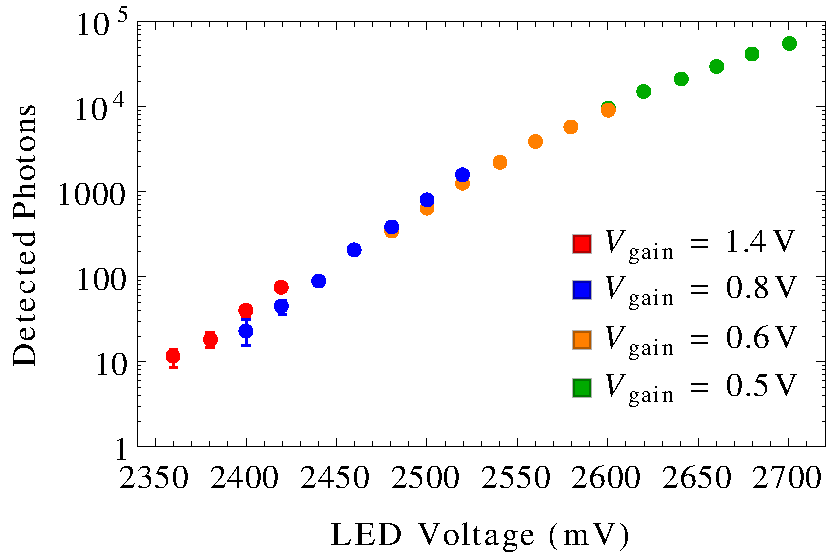
\includegraphics[width=\textwidth]{pmttest}
    \end{subfigure}%
    \begin{subfigure}{0.49\textwidth}
        \caption{After potting.}
        \label{fig:pmtafterpotting}
        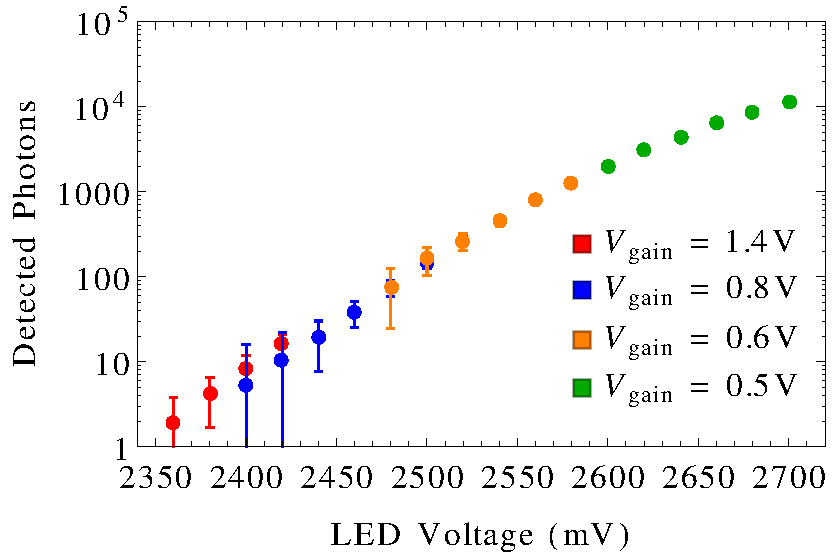
\includegraphics[width=\textwidth]{pmttest_potted}
    \end{subfigure}
    \caption{Tag PMT response measured at various different gains and photon fluxes. A calibrated LED was placed 50\,cm from the face of the PMT and pulsed for 50\,ns at various voltages that produced a known photon flux on the PMT.}
	\label{fig:calibratedled}
\end{figure}

\subsection{Hydrostatic test at Queen's}

\begin{figure}
\centering
\caption{}
\label{fig:pressurechamber}
\end{figure}

The Queen's pressure chamber was used to pressure test all SNO sources and was similarly used to pressure test the Cherenkov source. This pressure chamber is a 10" diameter aluminum cylinder that is pressurized with tap water pressure. For this test the Cherenkov source was removed from its radon proof bag and fully assembled in a clean room environment with viton o-rings. A 5/8" aluminum plug was used in place of an ubmilical. Because of the use of tap water extra care was taken to ensure the source would not be contaminated by isolating it from the bulk volume of water. The source was heat sealed into a bag of DI water and lowered into the pressure chamber which was also filled with DI water. After sealing the chamber it was pressurized to 60psi and the source remained at this pressure for one hour. This pressure exceeds the approximately 22psi pressure differential from mine pressure to the bottom of the acrylic vessel by a very conservative margin. To achieve this pressure approximately $0.5\%$ of the water inside the pressure chamber (but outside the sealed bag) was tap water. After depressurizing, the bagged source was removed from the pressure chamber and the bag was inspected to confirm there were no leaks into the tap water contaminated volume. The Cherenkov source was then removed from the DI water bag and was dried externally with grade 5.0 nitrogen gas in a clean room environment. 

To confirm that the Cherenkov source passed the pressure test, the source was disassembled in a clean room environment and inspected for water ingress. Neither the single o-ring seal at the steel-acrylic interface, the double o-ring seal at the umbilical flange, nor the double o-ring seals at the umbilical showed any sign of a water leak. With this result the source passed the pressure test. The source was then returned to its radon proof bag, flushed with nitrogen, and stored to await final cleaning and deployment.

\section{Water Phase Analysis}
\label{chap:water_phase}

\subsection{Data Taking}
The Cherenkov source was deployed in SNO+ water phase to calibrate the optical output of the source relative to the $^16$N source.
In total 18 hours of data were taken with the source deployed and \Li being injected into the decay chamber.
The PMT tag signal was connected to an empty PMT channel of the SNO+ electronics (FECD) to integrate the resulting pulses for event tagging.
In addition, the PMT signal was connected to the trigger signal digitizer (CAEN) in the SNO+ tigger system to record the full pulse.
During this deployment we discovered the gas connections were not ideal for connecting to SNO umbilicals, which leaves some room for improvement for future deployments.

\subsection{Data Cleaning}
In water phase there is no expected contamination from Bremsstrahlung gammas, however, since the detector is self triggering during deployment, tagged events must be identified and separated from other unrelated detector triggers.
This is done by characterizing the signal from the tag PMT contained within the source.
For a perfect event, the alpha scintillation within the source will result in a large signal with a long time constant.
There is some contamination from \Li betas which clip the PMT prior to exiting the source which should be excluded.


\begin{figure}
\centering
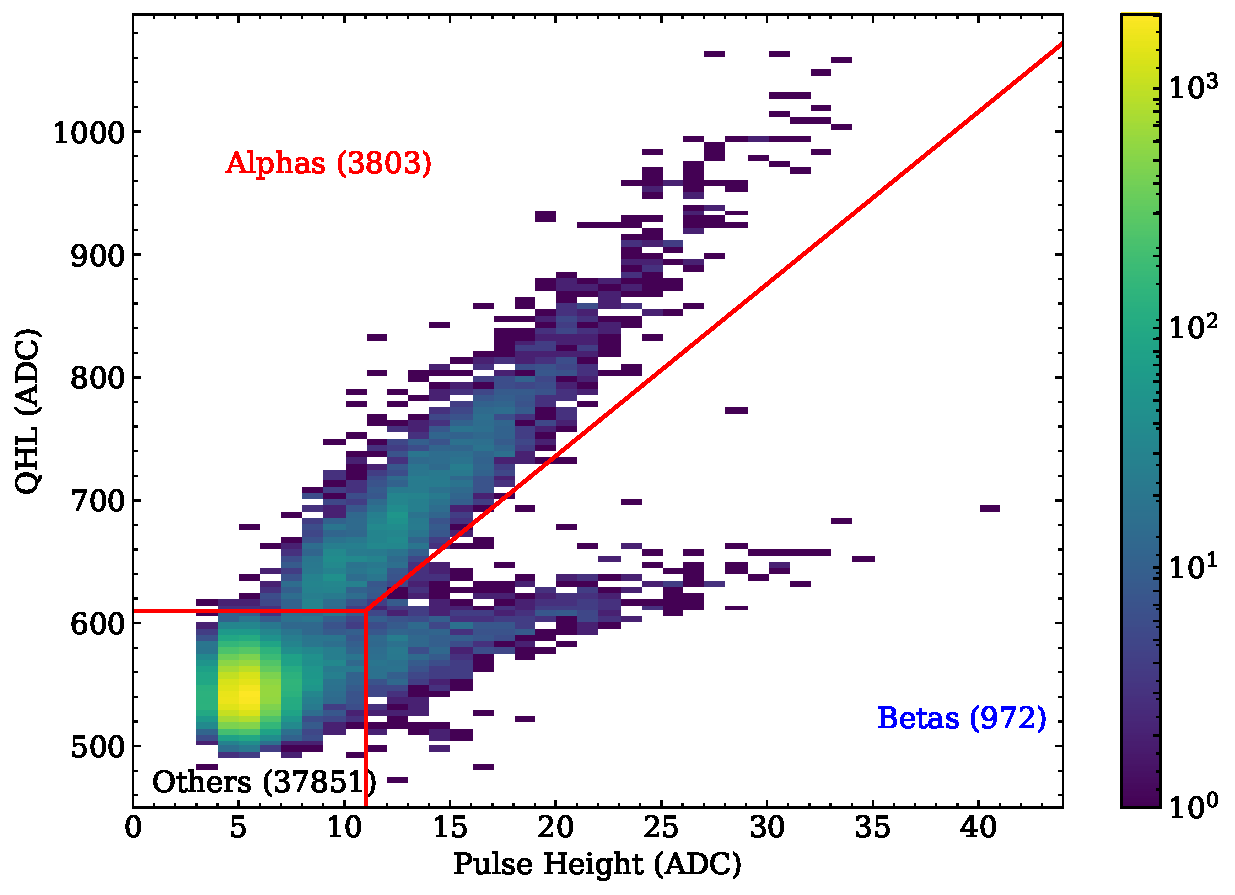
\includegraphics[width=0.8\columnwidth]{data_tagging}
\caption{\label{fig:chsrc_classify} Shown here are all events where the tag PMT crossed threshold during detector triggers during source deployment. Note the tag threshold was set quite low, resulting in a population of "other" events inconsistent with true alphas or beta contamination. Red lines show nominal cut values used in classification.}
\end{figure}

These events can be well separated in a 2D histogram of total charge (QHL) vs pulse height from the tag PMT. 
Classifications of events with nominal cuts are shown in \Cref{fig:chsrc_classify}.
The population of "other" events are those in which the detector issued a trigger unrelated to the Cherenkov source, and hence no light was seen by the tag PMT.
The distribution of number of hit PMTs in the detector for each of these classifications is shown in \Cref{fig:chsrc_nhits} while \Cref{fig:chsrc_pmttraces} shows the average digitized trace for each class.
The alphas have an nhit distribution nominally consistent with MC expectations, and a large tag trace with a long tail consistent with alpha scintillation light.


\begin{figure}
\centering
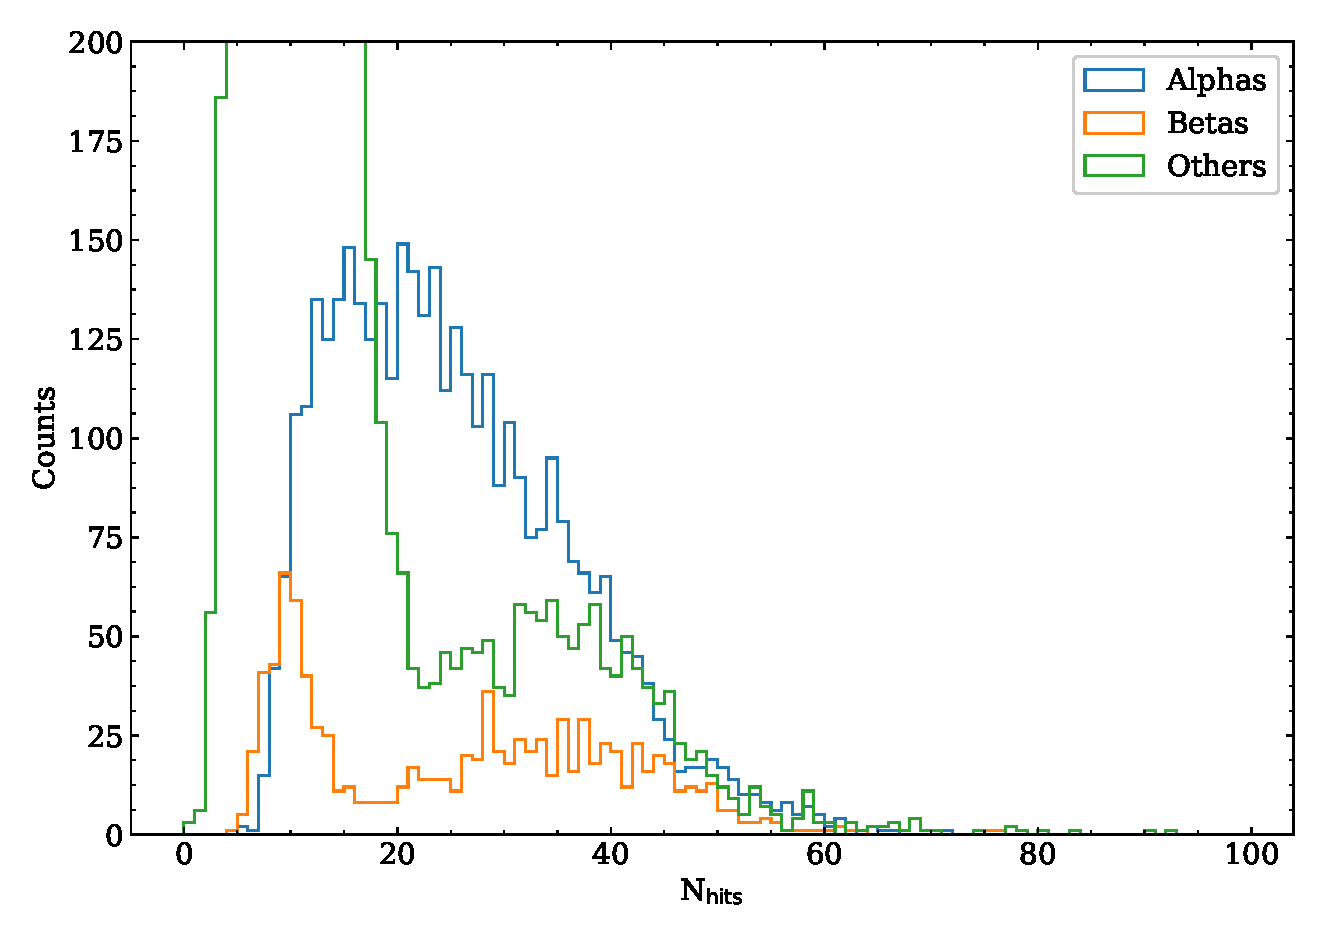
\includegraphics[width=0.5\columnwidth]{nhit_dists}
\caption{\label{fig:chsrc_nhits} The hit PMT distributions for the different classifications of Cherenkov source data.}
\end{figure}


\begin{figure}
\centering
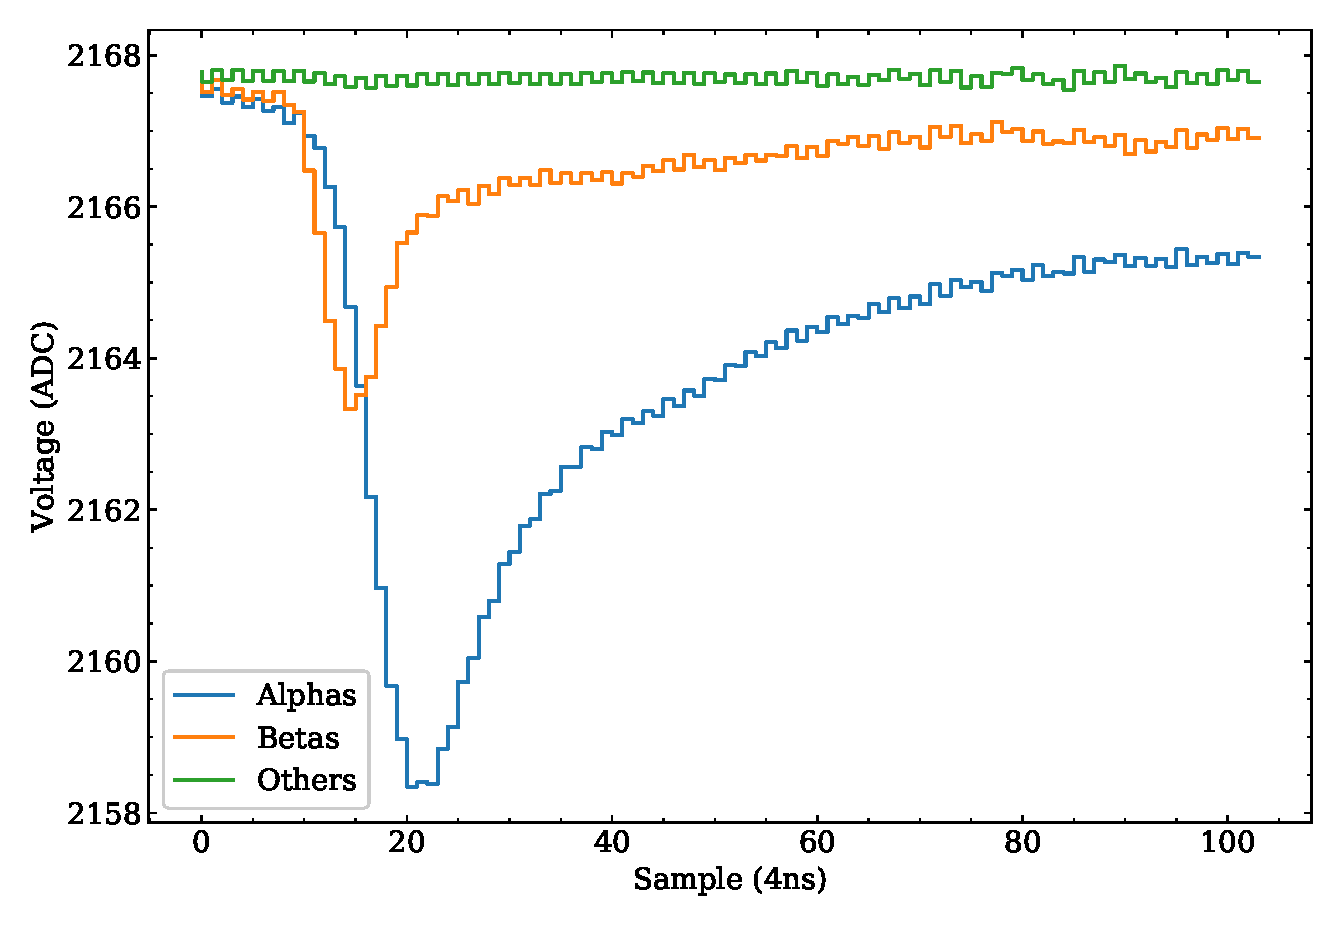
\includegraphics[width=0.5\columnwidth]{average_traces}
\caption{\label{fig:chsrc_pmttraces} The average tag PMT traces from the different classifications of Cherenkov source data.}
\end{figure}

\subsection{Collection Efficiency Fit}
The most straightforward way to extract the correction factor to the MC collection efficiency is to varry that efficiency in MC to maximize the Poisson likelihood of the data.
MC is generated with an $^16$N calibrated photon collection efficiency $C_{eff_0}$.
This quantity is scanned over a range of collection efficiencies while a MC model of the source is used to predict a hit PMT distribution.
To avoid accounting for detector trigger efficiencies, only events with $>20$ hits -- where trigger efficiency is garunteed to be 100$\%$ -- are included in this analysis.
At each point in the scan the negative logarithm of the Poisson likelihood of the data is calculated resulting in a best fit at $0.945^{+0.015}_{-0.015}$ $C_{eff}/C_{eff_0}$ where the errors are statistical only.
The scan itself is shown in \Cref{fig:chsrc_scan} with the best fit hit PMT distribution in \Cref{fig:chsrc_bestfit}.
This indicates a systematic offset between the light emission of the MC model of the source and the actual source of roughly $5\%$, which should be taken into account when calibrating future phases of SNO+.

\begin{figure}
\centering
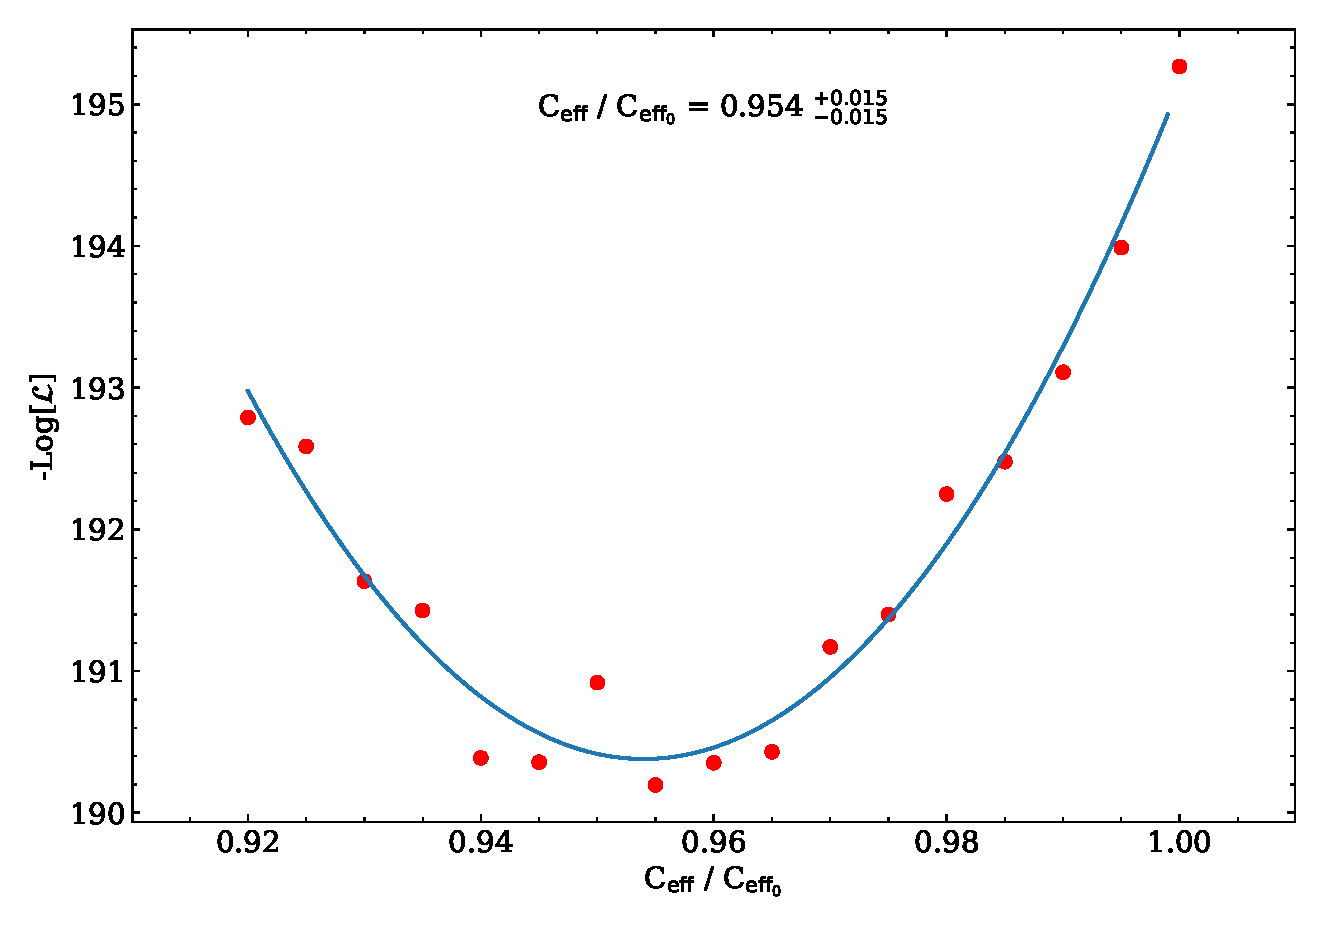
\includegraphics[width=0.5\columnwidth]{100k_bulk_py_ceff_scan}
\caption{\label{fig:chsrc_scan} A plot of the region around the minimmum negative log likelihood space in the collection efficiency scan for calibrating the Cherenkov source.}
\end{figure}

\begin{figure}
\centering
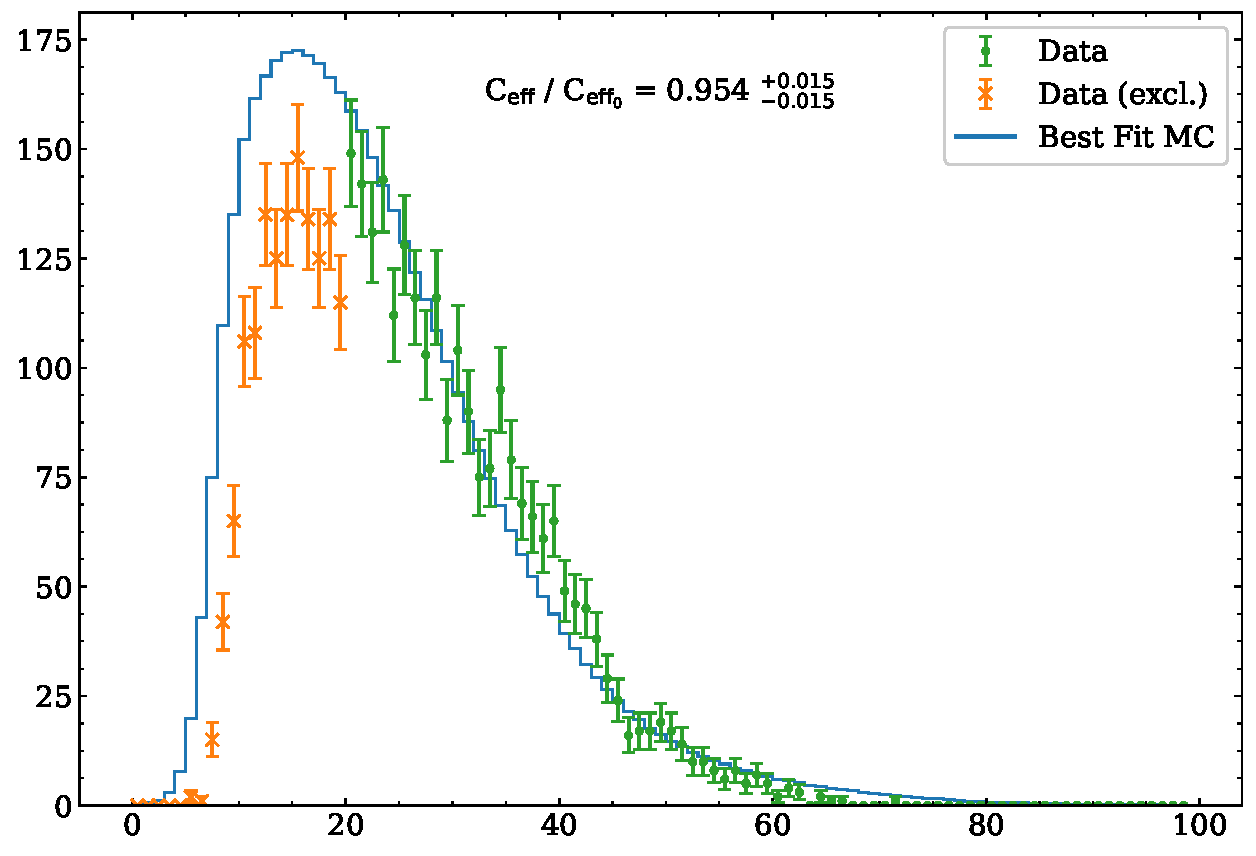
\includegraphics[width=0.5\columnwidth]{100k_bulk_py_ceff_scan_bestfit}
\caption{\label{fig:chsrc_bestfit} A comparison between data and simulation for the best fit collection efficiency in the water phase deployment for the Cherenkov source.}
\end{figure}

